\chapter{Antecedentes}
\label{chap:antecedentes}

\drop{E}{n} este capítulo se muestra el trabajo de documentación e investigación previa a la realización del presente \ac{TFG}. En primer lugar se abordarán los sistemas de posicionamiento, su historia y el desarrollo del gps\footnote{Debido al extendido uso de la denominación \textit{gps} como sinónimo de los \ac{GNSS}, se escribirá en minúsculas en referencia a los citados sistemas. Para referirse al sistema de posicionamiento propiedad del gobierno de los Estados Unidos \acf{GPS} se utilizará el acrónimo en mayúsculas}  y los antecedentes de los \ac{SIG}, más tarde se comentarán algunos aspectos relevantes de la web y de las tecnologías móviles. Para terminar, se enumerarán algunas aplicaciones similares que podemos encontrar actualmente en el mercado.

\section{Localización geográfica y \acf{SIG}}

%HISTORIA DEL GPS
Los \ac{GNSS} permiten conocer en tiempo real la posición de un objeto cualquiera en la superficie terrestre.

Según Scott Gleason y Demoz Gebre-Egziabher \cite{Glea09} podríamos definir la navegación como:

	\vspace{5mm}
\begin{tikzpicture}
	\node[shadowBox] {El proceso de determinación de la posición, la velocidad y, en algunos casos, la orientación de un objeto.};
\end{tikzpicture}
	\vspace{5mm}

Por tanto, un \ac{GNSS} consiste en una constelación de satélites que permiten determinar con precisión las coordenadas geográficas y la altitud de un punto dado en cualquier punto de la superficie terrestre.

El inicio de este tipo de sistemas podríamos encontrarlo en los primeros marinos. La decisión de alejarse de las rutas que transcurrían a lo largo de la línea de visión de la costa, con la intención de reducir el tiempo, los costes derivados de los viajes y la posibilidad de encontrar nuevos mercados, planteó un nuevo reto tecnológico consistente en conocer con exactitud la localización en la que se encontraban.

En cualquier ámbito de navegación, no solamente en el marítimo, el viajero necesita determinar su posición con respecto a un punto fijo, de manera que pueda trazar una ruta correcta hacia su destino conociendo las posiciones de origen y destino. Los primeros intentos vienen de la mano de la bóveda celeste, conociendo que el sol sale por el este y se pone por el oeste no resultaba complicado fijar los puntos cardinales durante el día. Durante la noche, la estrella polar o \textit{Polaris} parece mantenerse fija en el cielo nocturno, mientras el resto de constelaciones van variando su posición según avanza la noche y apareciendo y desapareciendo con el curso de las estaciones. Esto es debido a que esta estrella, ubicada en la constelación de la \textit{Osa menor} o \textit{Ursa Minor} se encuentra parcialmente alineada con el eje de rotación de la tierra, lo que hace que cualquier observador desde la corteza terrestre tenga la sensación de que la estrella se encuentra en aparente inmovilidad en la bóveda celeste, marcando precisamente el punto cardinal norte. Este fenómeno se da únicamente en el hemisferio norte, ya que en el hemisferio sur no puede observase la constelación citada. Para conseguir el mismo efecto en el hemisferio austral, se utiliza la \textit{Cruz del Sur}, que señala hacia el polo sur.\\

Los antiguos marinos nórdicos, descubrieron un tipo de calcita incolora y transparente, extraído del fiordo de Reydarfjördur en el este de Islandia y también conocido como espato de Islandia. Este material posee una propiedad física llamada birrefringencia, consistente en el desdoblamiento de las partículas de luz incidentes en dos rayos independientes conocidos como rayo ordinario (por seguir las normas de dirección de la refracción) y rayo extraordinario (con índices variables en la refracción y velocidad de los fotones), siendo estos dos rayos perpendiculares entre sí (\cite{Aug08}). Esto se traduce en que si se escribe una palabra y se coloca un trozo de este mineral encima se observará el texto dos veces (ver figura \ref{fig:iceland_calcite}).\\

\begin{figure}[h!btp]
\centering
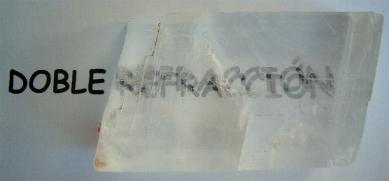
\includegraphics[scale=0.5, fbox={\fboxrule} 4mm]{images/03-antecedentes/54-espato_islandia.jpg}
\caption{Espato de Islandia}
\label{fig:iceland_calcite}
\end{figure}

Mediante esta propiedad, y dibujando un elemento en el cuerpo del cristal, se puede determinar la posición del sol fácilmente, independientemente de la existencia de nubes o incluso con el cuerpo celeste bajo el horizonte, simplemente fijándose en la intensidad de la sombra de los dos cuerpos que se observarán. Cuando las intensidades sean similares quedará fijada la posición de la fuente de luz.\\


Otras soluciones más precisas vinieron de la mano de un gran conocimiento de la bóveda celeste y la posición de las estrellas. Usando instrumentos como el astrolabio y el sextante (ver figura \ref{fig:sextante_astrolabio}), se podía calcular con asombrosa exactitud la posición.

\begin{figure}[h!btp]
	\begin{adjustbox}{minipage=\linewidth, fbox}
		\centering
		\subfigure[Sextante]{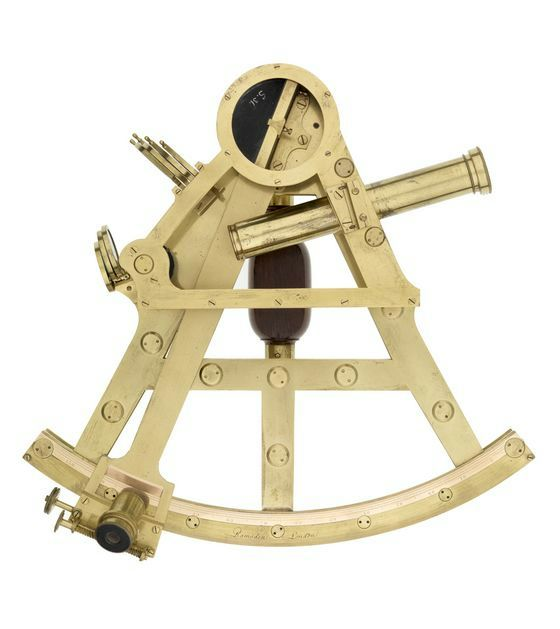
\includegraphics[width=60mm, height=80mm]{./images/03-antecedentes/04-sextante.png}}
		\hspace{10mm}
		\subfigure[Astrolabio]{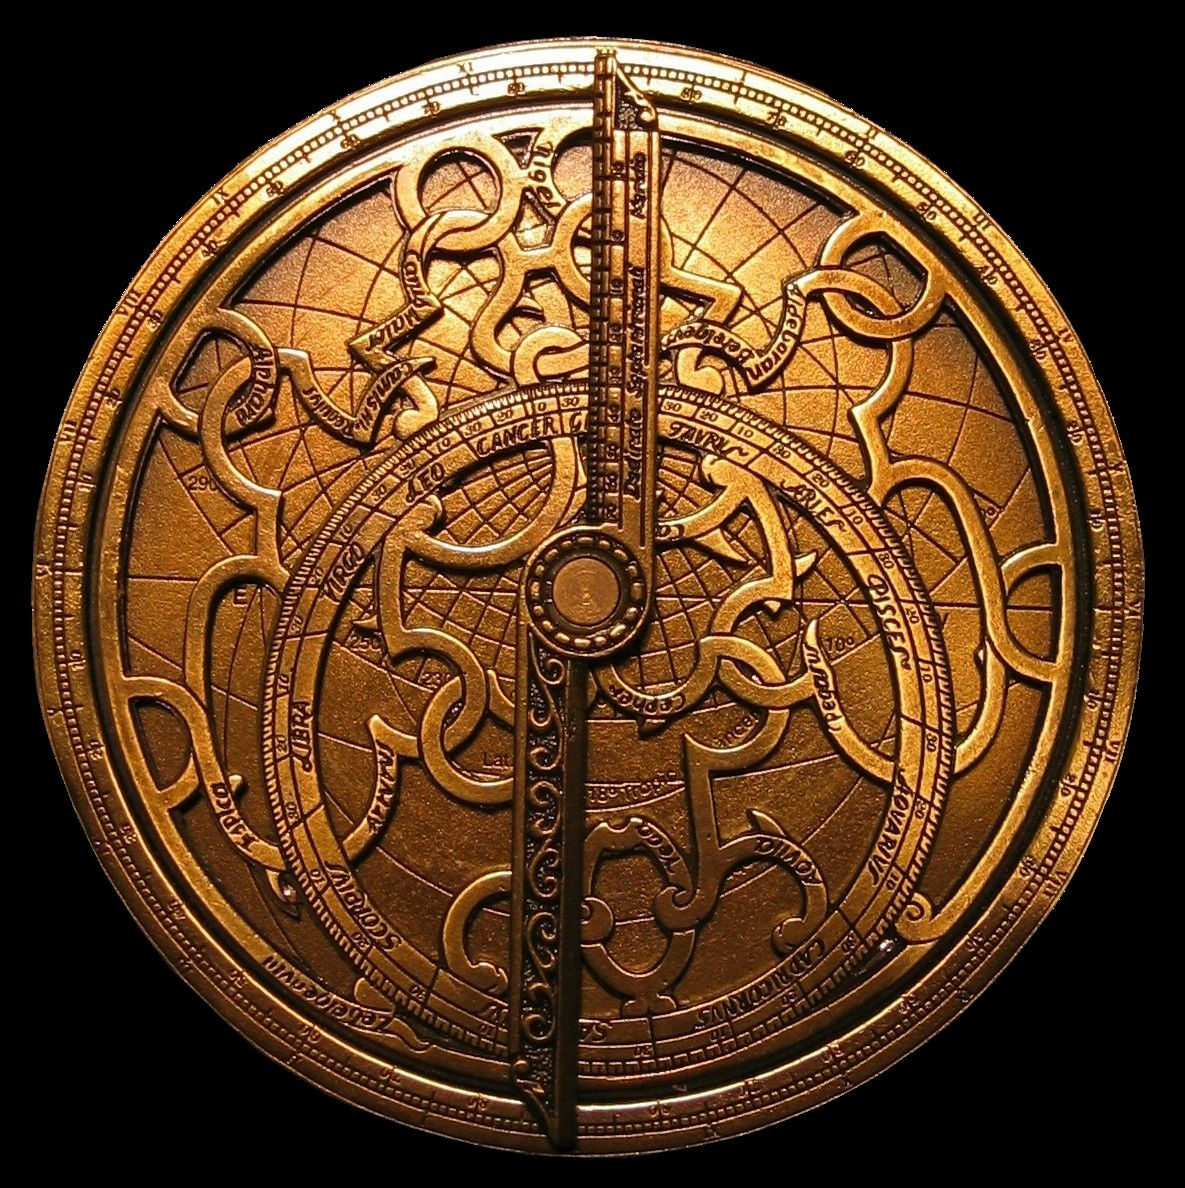
\includegraphics[height=80mm]{./images/03-antecedentes/05-astrolabio.png}}
	\end{adjustbox}
	\caption{Primeros instrumentos de navegación}
	\label{fig:sextante_astrolabio}
\end{figure}

El gran problema se encontraba cuando no podía observarse la bóveda celeste, debido principalmente a la climatología. Para ello se desarrolló la brújula. 
La primera referencia que tenemos de este invento se produce en unos escritos chinos del siglo XI. Esta primera brújula tomaba la forma de una cucharilla sin mango, fabricada con magnetita que se dejaba flotar libremente en una vasija con agua, tomando la conocida orientación norte-sur, aunque más tarde se sustituyó el recipiente por un eje de rotación (ver figura \ref{fig:chinese_compass}).
Posteriormente, Sir William Thomson (ver figura \ref{fig:william_thomson}), primer Barón Kelvin, conocido por la escala de temperatura homónima, la mejoró haciéndola inmune a la interacciones magnéticas de los barcos y el estado embravecido de las aguas. 

\begin{figure}[h!btp]
\centering
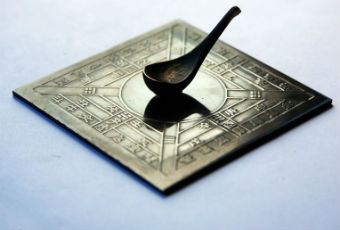
\includegraphics[scale=0.5, fbox={\fboxrule} 4mm]{images/03-antecedentes/53-chinese_compass.jpg}
\caption{Brújula china}
\label{fig:chinese_compass}
\end{figure}

\begin{figure}[h!btp]
	\begin{adjustbox}{minipage=\linewidth, fbox}
		\centering
		\subfigure[Sir William Thomson]{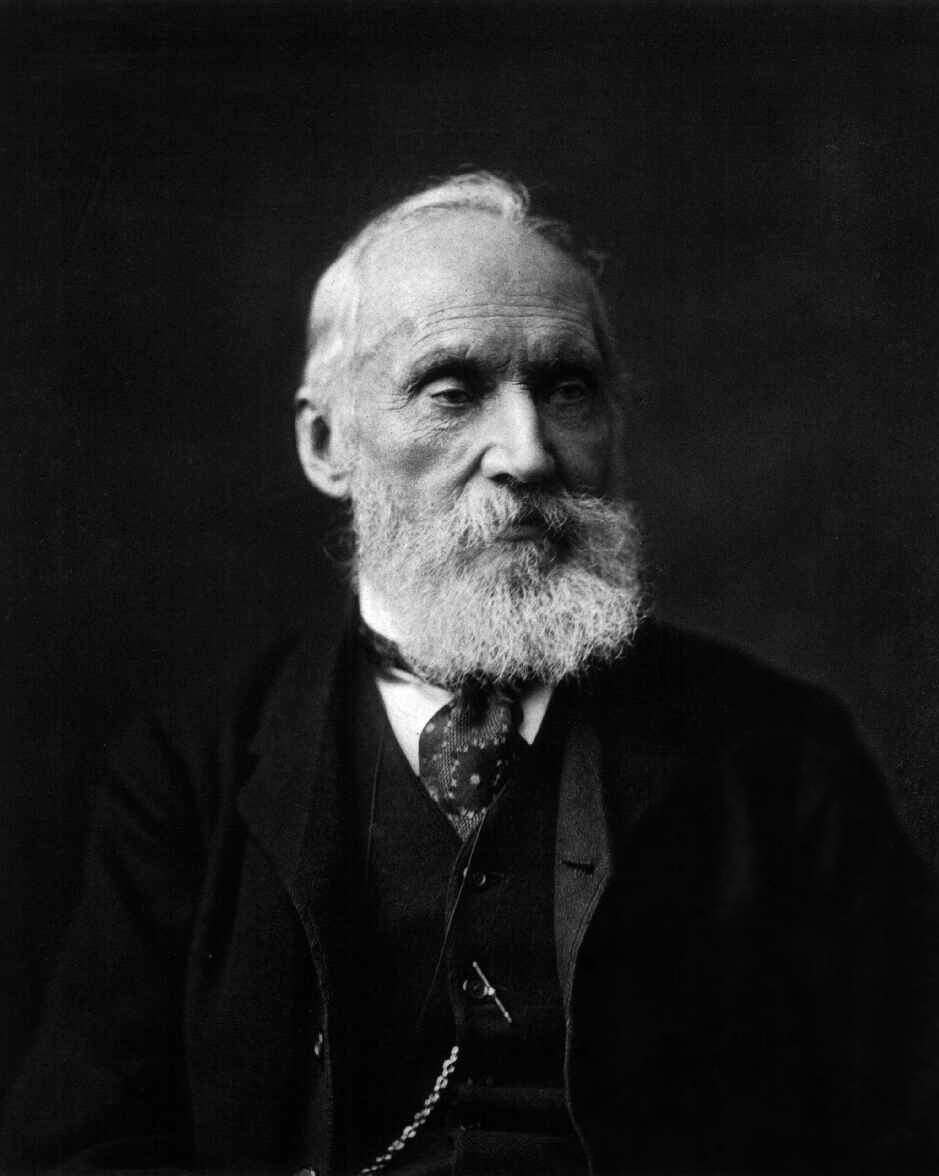
\includegraphics[width=60mm, height=80mm]{./images/03-antecedentes/51-william_thompson.jpg}}
		\hspace{10mm}
		\subfigure[Brújula]{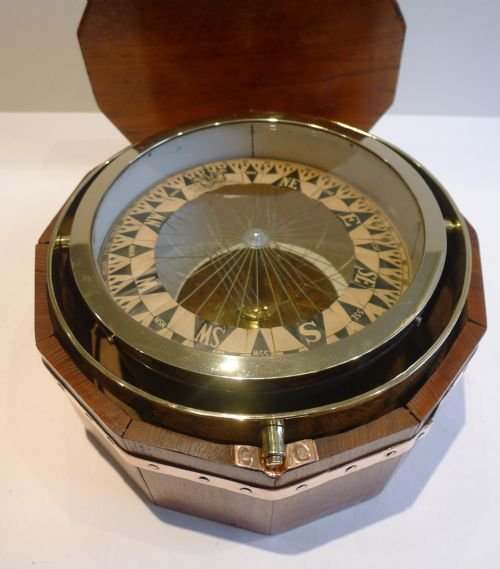
\includegraphics[height=80mm]{./images/03-antecedentes/52-william_thomson_compass.jpg}}
	\end{adjustbox}
	\caption{Sir William Thomson y su brújula}
	\label{fig:william_thomson}
\end{figure}



Hasta tiempos recientes (segunda mitad del S. XX), con la irrupción del posicionamiento satelital, este era el método usado para conocer la ubicación en la que se encontraban.
Los primeros prototipos del gps se desarrollan a principios del S. XX, coincidiendo con los comienzos de la automoción, aspecto este último que ha dado la gran fama que posee actualmente esta tecnología.
El primer gps data de 1909, que consistía en un odómetro que giraba un mapa indicando los hitos más importantes que se podían encontrar en el punto kilométrico en el que te encontrabas.
Este primer prototipo se llamaba \textit{Jones Live Map} (ver figura \ref{fig:jones_live_map}), cada mapa era válido para unos 160 km y después había que cambiarlo por el siguiente mapa. Este primer intento de gps dejó de fabricarse en los años 20, cuando las carreteras comenzaron a estar correctamente señalizadas \cite{GPS12}.

\begin{figure}[h!btp]
\centering
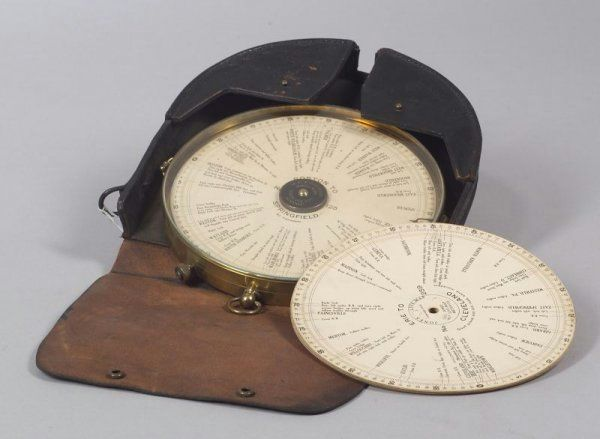
\includegraphics[scale=0.5, fbox={\fboxrule} 4mm]{images/03-antecedentes/06-jones_live_map.png}
\caption{Jones Live Map}
\label{fig:jones_live_map}
\end{figure}

También en la década de los veinte, hizo su aparición el \textit{Plus Fours Routefinder} (ver figura \ref{fig:plus_fours_routefinder}), consistente en un pequeño reloj de muñeca con una serie de papiros con la información de la ruta. Estos papiros debían ir desenrollándose de forma manual para seguir las indicaciones \cite{Plus14}.

\begin{figure}[h!btp]
\centering
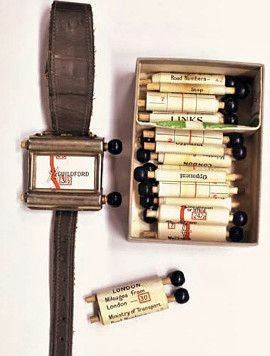
\includegraphics[scale=0.5, fbox={\fboxrule} 4mm]{images/03-antecedentes/07-plus_fours_routefinder.png}
\caption{Plus Fours Routefinder}
\label{fig:plus_fours_routefinder}
\end{figure}

Otro de los padres del gps moderno es el llamado \textit{Iter Avto} (ver figura \ref{fig:iter_avto}), consistente en un mapa enrollado conectado al velocímetro del coche para sincronizarlo. La dos grandes ventajas con respecto al \textit{Plus Fours Routefinder}, consistía en que se instalaba sobre el salpicadero del coche y mostraba de forma gráfica la posición. Su inconveniente, cualquier desviación de la ruta era completamente indetectable \cite{Parra13}.

\begin{figure}[h!btp]
\centering
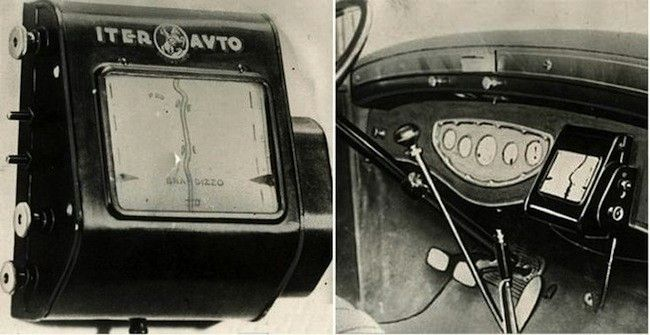
\includegraphics[scale=0.5, fbox={\fboxrule} 4mm]{images/03-antecedentes/08-iter_avto.png}
\caption{Iter Avto}
\label{fig:iter_avto}
\end{figure}

Durante la segunda guerra mundial, la \ac{RAF} desarrolló un sistema de
posicionamiento para sus bombarderos consistente en tres estaciones de radar que localizaban
con precisión al avión \cite{Ori13}. 
Los verdaderos orígenes de los gps como sistema de navegación satelital se remontan a 1957 con
el programa \textit{TRANSIT}. Por un lado la marina de los \ac{EE.UU.} inicia el programa \textit{Polaris},
que consiste en el despliegue de misiles transcontinentales suboceánicos. Alcanzar los objetivos señalados
con los misiles dependía de la capacidad de determinar con precisión la posición de los
submarinos en cualquier punto de la superficie terrestre. Por otro lado, la universidad Johns
Hopking de Maryland, consigue determinar con precisión la órbita del \textit{Sputnik 1} a partir del
desplazamiento Doppler sufrido por la señal que emitía y el conocimiento preciso de la posición
del receptor. Con estos elementos, invertir los términos del problema resultó relativamente
sencillo, esto es, conociendo la posición de un satélite de forma precisa, es posible determinar
la de un receptor situado en el submarino de posición desconocida midiendo el desplazamiento
Doppler sufrido por la señal emitida del satélite.

El sistema \textit{TRANSIT} entró en funcionamiento en 1964 con el lanzamiento de 10 satélites y se mantuvo en servicio
hasta 1996. En 1967 se permitió su uso civil. El error típico de este sistema era de unos 250
metros, por lo que resultaba muy útil para la navegación de aviones, barcos y submarinos, pero
por razones obvias (precisión y tamaño de los receptores) aún estaban lejos de los sistemas de
navegación personal actuales.

Mientras \ac{EE.UU.} desarrollaba el sistema \textit{TRANSIT}, la Unión Soviética había comenzado casi al mismo tiempo, un sistema muy parecido con idénticas prestaciones, el \textit{TSICADA}, lo que resultaba inadmisible para los norteamericanos en el
contexto de la guerra fría, por lo que comenzó a desarrollarse lo que posteriormente sería el
\ac{GPS} \cite{Pala10}.
El \textit{NAVSTAR-GPS} nació en 1973 para uso exclusivamente militar, con una constelación de 24
satélites en órbitas inclinadas de 12 horas, lo que se traducía en que cualquier receptor en el
mundo tendría en su horizonte visible al menos 5 satélites disponibles en todo momento. El
TRANSIT, no sólo no podía garantizar esto, debido a que sus satélites eran de órbita baja, si no
que con sus 6 satélites, algunos receptores podían estar varias horas esperando recibir señal. El primer
satélite de la constelación se puso en órbita en 1978. La precisión de este nuevo sistema era de 1 metro y podía
ser incorporado en misiles, bombas inteligentes, vehículos, etc. Debido a su consideración de
recurso de gran valor estratégico, su uso estaba limitado al ámbito estrictamente militar.
 El 31 de agosto de 1983 tuvo lugar uno de los incidentes internacionales más graves de la
guerra fría, que a la postre resultaría decisivo para el uso actual del \ac{GPS}, el derribo del vuelo de
\textit{Korean Airlines KAL007} por parte de la \ac{URSS} \cite{Kore15}.

El citado vuelo, usando los sistemas de navegación tradicionales disponibles en aquella época, y
usando el piloto automático, invadió en dos ocasiones el espacio aéreo de la Unión Soviética,
que acabó interceptándolo mediante dos cazas militares y derribándolo con un ataque con
misiles, matando al pasaje y la tripulación completa, con un resultado de 269 fallecidos.
La respuesta internacional no se hizo esperar, y el entonces presidente de \ac{USA}, Ronald Reagan,
anunció que el sistema \ac{GPS} estaría disponible para propósitos civiles una vez finalizase el
proyecto, con la intención de que no se volvieran a repetir incidentes similares.
 Para evitar que sus enemigos pudieran hacer uso de esta nueva tecnología para construir
misiles de precisión con los que atacarlos, el Departamento de Defensa de \ac{EE.UU.} impuso una
serie de restricciones en la precisión de los receptores, de manera que el error en el
posicionamiento fuera mayor que el de los disponibles para uso militar. Por ello los receptores de gps de uso
civil eran incapaces de mostrar una resolución menor a veinte metros.
Durante la primera guerra del golfo, en 1991, se desarrolló una mejora en la precisión del \ac{GPS}
llamada, \ac{GPS} Diferencial, que conseguía precisiones de entre 1 y 3 metros de exactitud.

\subsection{Funcionamiento de los gps}

La base sobre la que se asienta el funcionamiento del posicionamiento mediante satélites consiste en que sea cual sea nuestra localización en la corteza terrestre, siempre estaremos a la vista de al menos cuatro satélites distintos.

Cada uno de estos satélites transmite información acerca de su localización que será utilizada por nuestro receptor para calcular la distancia a la que se encuentran, en función del tiempo que tardan las señales en llegar.
Conociendo la distancia a la que se encuentran, como mínimo, tres satélites, es posible conocer con un cierto grado de aproximación la zona en la cual debemos estar posicionados. Este proceso de localización se conoce como triangulación.

Si estamos al alcance de un único satélite, la posible zona en la que nos encontraremos será todo el área de influencia del mismo. En el caso de utilizar dos satélites, la zona en la que podríamos encontrarnos sería la superficie de la intersección de las dos esferas imaginarias creadas con centro en cada uno de los satélites y radio la distancia a nuestra posición.

En el caso de utilizar tres satélites, que como se ha comentado anteriormente es el mínimo necesario, la posible localización se ve reducida a dos puntos. Para conocer con precisión cual de esos dos puntos es el correcto haría falta un cuarto satélite, pero en términos generales, uno de esos puntos no estará ubicado en la corteza terrestre, por lo que podrá descartase y conocer de esta manera nuestra localización (ver figura \ref{fig:triangulacion-satelital}).

\begin{figure}[h!btp]
\centering
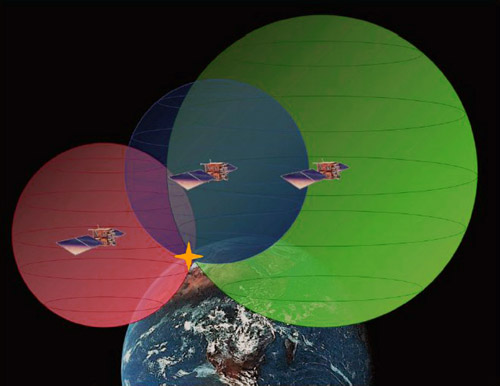
\includegraphics[scale=0.5, fbox={\fboxrule} 0mm]{images/03-antecedentes/31-funcionamiento_gps.jpg}
\caption{Triangulación satelital}
\label{fig:triangulacion-satelital}
\end{figure}

Debido a razones obvias de estrategia militar, la precisión dada por los satélites \ac{GPS} incluía un cierto grado de error aleatorio llamado \textit{disponibilidad selectiva}. Este error fue eliminado el 2 de mayo del año 2000. Habitualmente la precisión para usos civiles se veía limitada a 100 metros \cite{Corr00}.

\subsection{Cartografía y \acs{SIG} \protect\footnote{La labor de documentación está basada en: \cite{Diaz15}.} }

Antes de la aparición de la historia, esto es, antes de la constatación escrita de los acontecimientos, se produjo la aparición de los mapas. Estos estaban realizados con la intención de establecer distancias, recorridos y localizaciones de elementos de cierta importacia.

El mapa más antiguo del que se tiene noticia proviene de la antigua Babilonia y está fechado alrededor de 4500 años a.C. Actualmente está conservado en el Museo Británico (ver figura \ref{fig:mapa-babilonio}).

\begin{figure}[h!btp]
\centering
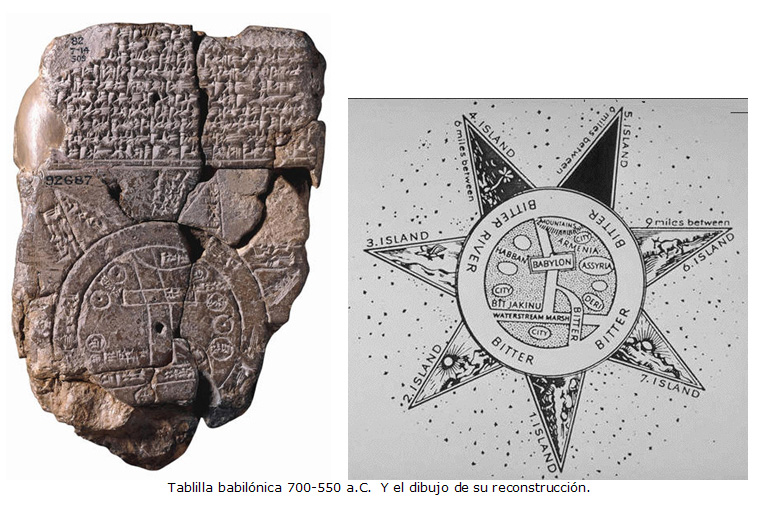
\includegraphics[scale=0.5, fbox={\fboxrule} 0mm]{images/03-antecedentes/32-mapa_babilonio.jpg}
\caption{Tablilla babilónica y reconstrucción}
\label{fig:mapa-babilonio}
\end{figure}

La antigua Grecia fue quien colocó las bases para la cartografía actual, aportando grandes conocimientos geométricos, matemático geográficos y  astronómicos. Los cartógrafos griegos, que admitían la forma esférica de la tierra, fueron los iniciadores del sistema de localización geográfica, es decir, las latitudes y longitudes, hicieron las primeras proyecciones \cite{Schl07} y dieron una cifra bastante aproximada del tamaño de nuestro planeta \cite{Aup09}.

Prácticamente todo lo que conocemos de la cartografía de este tiempo se debe a los escritos de Herodoto y Estrabón que mencionan a Anaximandro de Mileto como el realizador de un mapa completo de la tierra incorporando mares y ríos \cite{Kap10}. Pero de entre todos los personajes de la antigua Grecia, fue Claudio Ptolomeo el más importante para el campo de la cartografía con su obra \textit{Geographia} en la que puede apreciarse un mapamundi que abarca desde las islas Canarias por el oeste hasta China por el este (ver figura \ref{fig:mapa-ptolomeo}). Debido a que en este mapa aparecen las latitudes, el ecuador, la escala y está orientado al norte, es posible apreciar las bases de las cartas de navegación modernas.

\begin{figure}[h!btp]
\centering
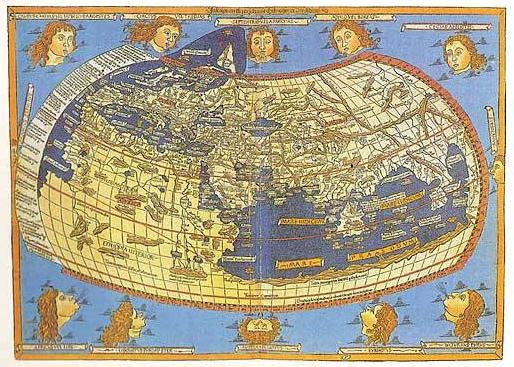
\includegraphics[width=120mm, fbox={\fboxrule} 0mm]{images/03-antecedentes/33-mapa_ptolomeo.jpg}
\caption{Mapa Ptolemáico}
\label{fig:mapa-ptolomeo}
\end{figure}

Durante la era romana se sufrió un enorme retroceso en la cartografía, que no volvería a los niveles griegos hasta el siglo XVI, debido a que estaban más interesados en la realización de mapas prácticos para fines militares, administrativos y comerciales que en plasmar la realidad sobre el papel.

Durante la edad media, se pierde el concepto de esfera en los mapas y se representa el mundo ateniéndose más a conceptos místicos y religiosos que a la propia realidad. Normalmente aparece Jerusalén en el centro del mapa. Como ejemplo en la figura \ref{fig:mapa-beato-liebana} se puede observar el mapamundi de Beato de Liébana.

\begin{figure}[h!btp]
\centering
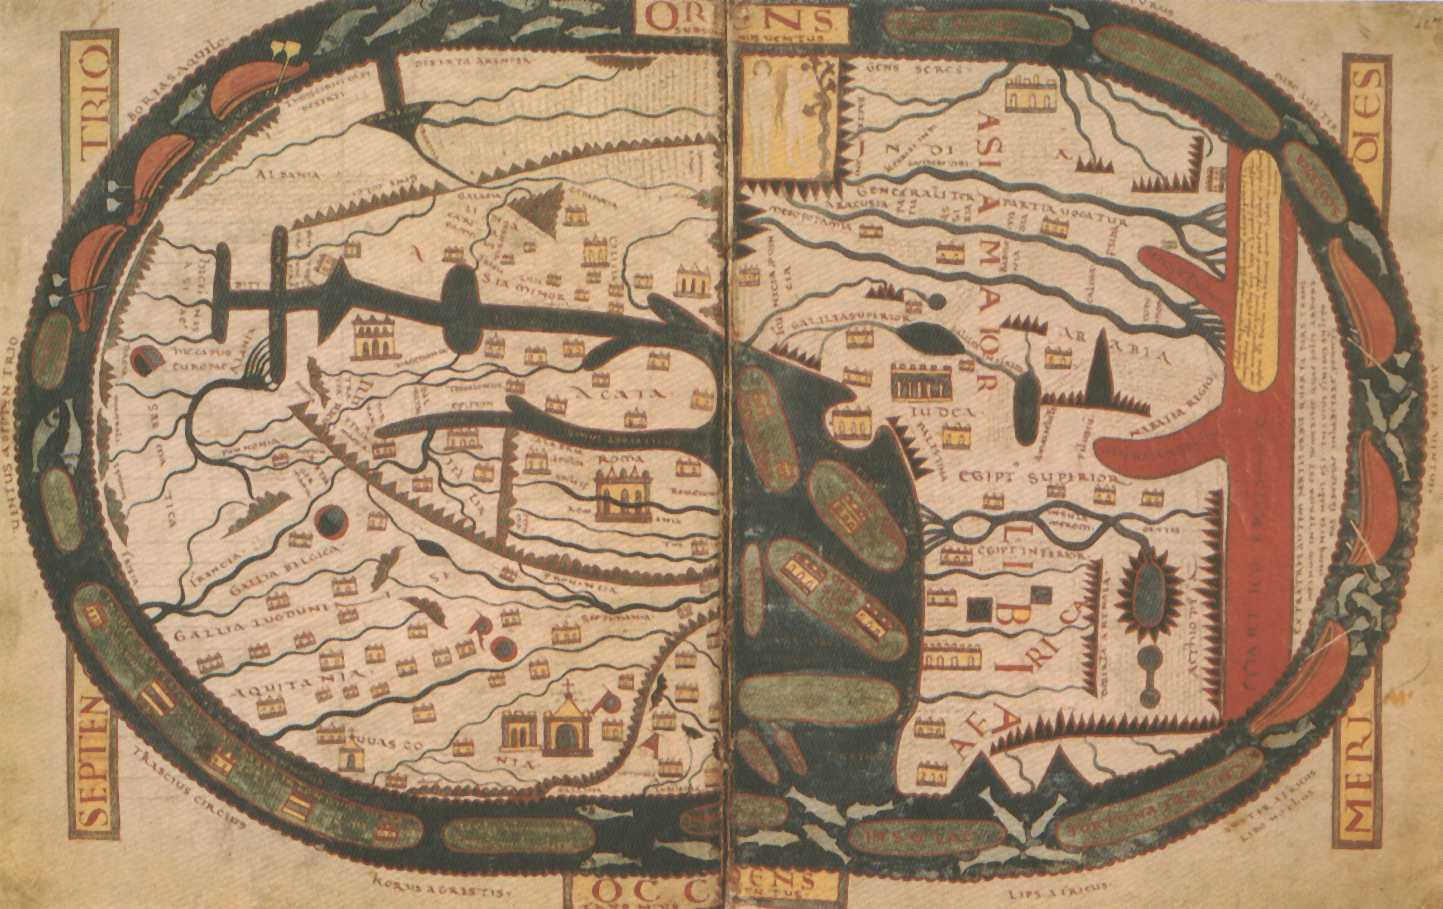
\includegraphics[width=160mm, fbox={\fboxrule} 0mm]{images/03-antecedentes/34-mapa_beato_liebana.jpg}
\caption{Mapamundi de Beato de Liébana}
\label{fig:mapa-beato-liebana}
\end{figure}

En el año 1154, Al Idrisi, cartógrafo ceutí, presenta un mapa alejado de las convenciones europeas existentes en la época y más cercano a los planteamientos griegos. En su mapa se puede observar con gran detalle los perfiles de Europa, norte de África y gran parte de Asia, aunque está orientado hacia el sur, en lugar de la orientación norte a la que estamos acostumbrados (ver figura \ref{fig:mapa-al-idrisi}).

\begin{figure}[h!btp]
\centering
\includegraphics[width=160mm, fbox={\fboxrule} 0mm]{images/03-antecedentes/35-mapa_al_idrisi.jpg}
\caption{Mapamundi de Abu Abd Allah Muhammad al-Idrisi. 1154}
\label{fig:mapa-al-idrisi}
\end{figure}

A mediados del siglo XV da comienzo la cartografía moderna como consecuencia de la recuperación de los escritos de Ptolomeo, la invención de la imprenta y la posibilidad de divulgar los mapas con facilidad. Los grandes avances técnicos respecto a la brújula y las embarcaciones, permitían hacer viajes más largos, por lo que se necesitaban mejores cartas de navegación.

En el año 1500 aparece el mapa de Juan de la Cosa, y aunque no existe consenso al respecto, la mayor parte de los autores consideran que éste es el primer mapa en que aparece América \cite{Verl06}, aunque hay que esperar al año 1507 para poder ver el nuevo continente con su nombre, propuesto por Americo Vespucio, en el mapa de Martin Waldseemüller (ver figura \ref{fig:mapas-america}).

\begin{figure}[h!btp]
	\begin{adjustbox}{minipage=\linewidth, fbox}
		\centering
		\subfigure[Mapamundi de Juan de la Cosa. 1500]{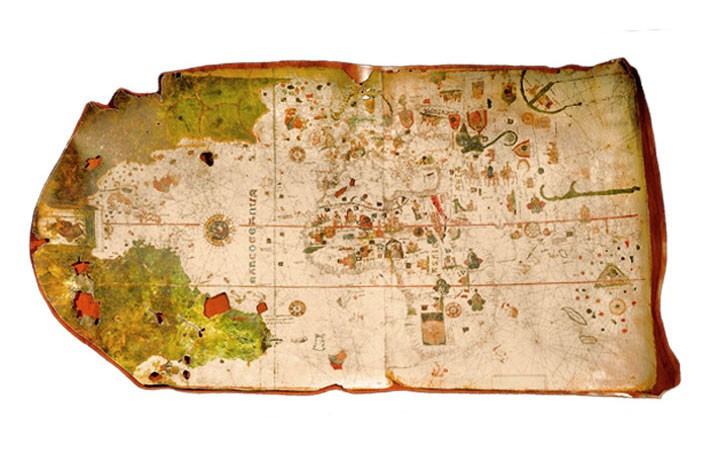
\includegraphics[scale=0.5]{./images/03-antecedentes/36-mapa_juan_de_la_cosa.jpg}}
		\hspace{10mm}
		\subfigure[Mapamundi de Martin Waldseemüller. 1507]{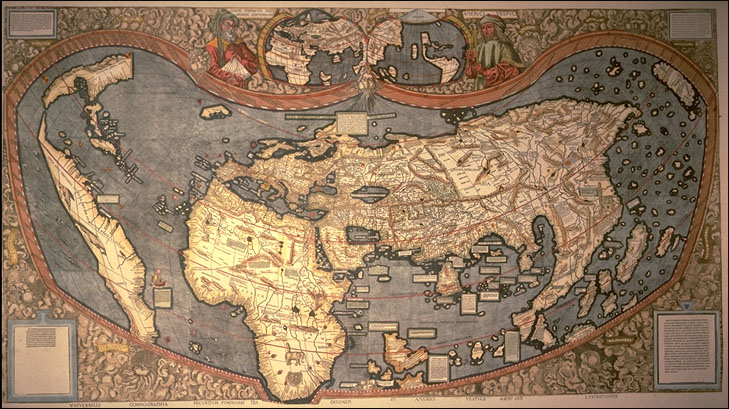
\includegraphics[height=80mm]{./images/03-antecedentes/37-mapa_martin_waldseemuller.jpg}}
	\end{adjustbox}
	\caption{Primeros mapas de América}
	\label{fig:mapas-america}
\end{figure}

Ya en el siglo XX, el desarrollo de la fotografía y la aviación, en el contexto de la Gran Guerra y sobre todo durante la Segunda Guerra Mundial, permitió una gran revolución cartográfica. Siendo conscientes de la gran ventaja militar que suponía un profundo conocimiento del terreno, empiezan a desarrollarse grandes proyectos en este sentido, que culminarán durante la segunda mitad del siglo en la cartografía de precisión mediante satélites \cite{Lind06}.

Debido a que el término \ac{SIG} engloba la integración de muy diversas áreas, no existe una única definición totalmente consensuada \cite{Chr97}. La definición aportada por el \ac{NCGIA} resulta ampliamente aceptada:

\vspace{5mm}
\begin{tikzpicture}
	\node[shadowBox] {
	Un SIG es un sistema de hardware, software y procedimientos elaborados para facilitar la obtención, gestión, manipulación, análisis, modelado, representación y salida de datos espacialmente referenciados, para resolver problemas complejos de planificación y gestión.};
\end{tikzpicture}
\vspace{5mm}

Uno de los elementos relevantes de los \ac{SIG} son la asociación de información a una imagen concreta y una de las primeras muestras de esto lo podemos encontrar en el Londres victoriano de mediados del siglo XIX. En el año 1854, el doctor John Snow (ver figura \ref{fig:john_snow}) utilizó un mapa del Soho londinense para ubicar los casos de un brote de cólera (ver figura \ref{fig:cholera_map}). Con la ayuda de los registros del hospital de Middlesex y de Henry Whitehead, párroco local, recogió las defunciones producidas mediante unas finas líneas de color negro que se apilaban unas sobre otras a medida que se producían las muertes, consiguiendo el efecto de asociación de información a imagen comentado en el párrafo anterior \cite{Cai11} (ver figura \ref{fig:cholera_map}).

\begin{figure}[h!btp]
\centering
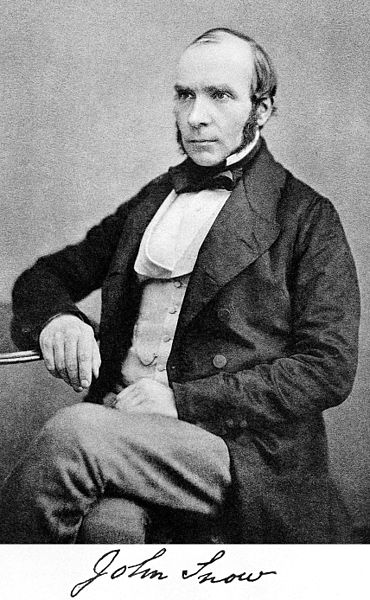
\includegraphics[scale=1, fbox={\fboxrule} 0mm]{images/03-antecedentes/02-john_snow.jpg}
\caption{Doctor Sir John Snow}
\label{fig:john_snow}
\end{figure}

\begin{figure}[h!btp]
\centering
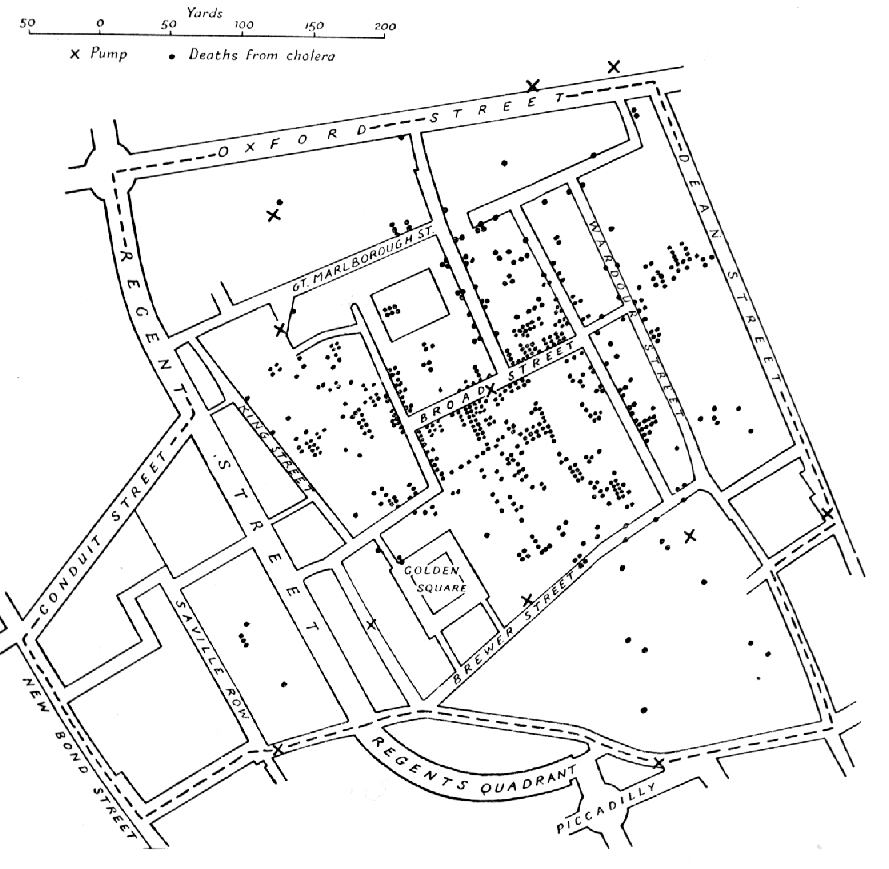
\includegraphics[scale=0.5, fbox={\fboxrule} 4mm]{images/03-antecedentes/01-cholera_map.jpg}
\caption{Mapa del Soho con los casos de fallecimiento por cólera}
\label{fig:cholera_map}
\end{figure}

Gracias a ello y referenciando en el mapa la posición de los pozos de agua, pudo comprobar como una gran cantidad de víctimas se encontraban dentro de la zona de influencia de una bomba de agua en Broad Street (ver figura \ref{fig:cholera_map_detail}), que a la postre resultó estar contaminada con heces. Recomendando la clausura de la misma consiguió acabar con la epidemia      \cite{Gunn07}. Debido a estos logros se le considera el padre de la epidemiología moderna y podemos ilustrar uno de los primeros ejemplos del uso de los \ac{SIG}.

Este ejemplo temprano, combinado con la geolocalización nos permite identificar las líneas base de la representación de elementos de lo que será el presente \ac{TFG}.

\begin{figure}[h!btp]
\centering
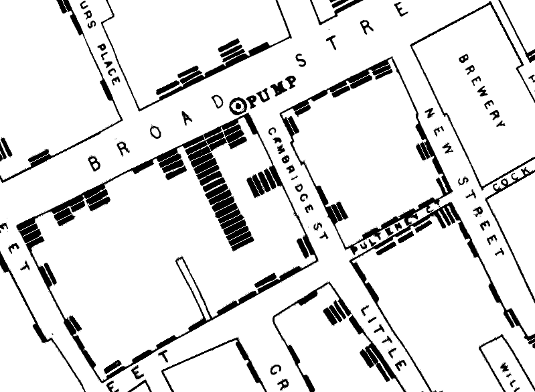
\includegraphics[scale=0.5, fbox={\fboxrule} 4mm]{images/03-antecedentes/03-cholera_map_detail.png}
\caption{Detalle del mapa del Doctor Snow}
\label{fig:cholera_map_detail}
\end{figure}

\section{Internet y la \ac{www}}

%Historia de Internet
Internet puede considerarse como una de las tecnologías que más ha cambiado el mundo y la que más rápidamente lo ha hecho. Gracias al nuevo concepto que supone, se puede acceder rápidamente a la mayor cantidad de información nunca antes recopilada en la historia de la humanidad.\\

La gran biblioteca de Alejandría, la mayor de las bibliotecas del mundo antiguo, contenía, antes de su destrucción unos 200.000 volúmenes, según Flavio Josefo, y calculaban que todo el conocimiento de la humanidad ocuparía un total de 500.000 volúmenes  \cite{Jos94}. Autores modernos han reconsiderado el posible número de volúmenes, aportando una cifra de unos 50.000 rollos, que podría equivaler a unos 12.500 libros actuales \cite{Esco01}.\\

Los Archivos Secretos Vaticanos contienen un total de 1.600.000 volúmenes \cite{Bav15}, la biblioteca nacional de España 28 millones \cite{Sanz15} y la biblioteca del congreso de los \ac{EE.UU.} 160 millones de documentos \cite{Libr15}. Comparando las cifras de algunas de las mayores bibliotecas del mundo con el número de documentos existentes en Internet, podemos hacernos una idea de lo que esta tecnología ha supuesto para la humanidad, no solamente en el volumen de información existente, si no en la facilidad de acceso a los mismos. En el año 2012, en Internet existían un total de 8310 millones de documentos accesibles.

Aunque no es lícito comparar estas cifras en bruto, ya que tal la cantidad no siempre está relacionada con la calidad, como dijo el escritor Neil Gaiman \cite{Gaim10}:

\vspace{5mm}
\begin{tikzpicture}
	\node[shadowBox] {
	Google puede devolverte cien mil respuestas, un bibliotecario puede devolverte la correcta.};
\end{tikzpicture}
\vspace{5mm}

En el año 1958 la compañía Bell crea el primer módem, un dispositivo capaz de transmitir datos binarios utilizando una línea telefónica (ver figura \ref{fig:bell_modem}). En el año 1962 J.C.R Licklider describe su concepto de \textit{Red galáctica}, consistente en una red interconectada globalmente que permitiera acceder a todo tipo de datos y programas desde cualquier sitio. Un año antes, en 1961, Leonard Kleinrock publicó su tesis doctoral acerca de la teoría de colas, que sería publicada como libro en el año 1964 (\cite{Klei64}) y que sirvió de fundamento a la teoría de conmutación de paquetes. Los datos se troceaban en partes, llamados \textit{paquetes}, a los que se les asignaba un número de secuencia antes de enviarlos. De esta manera, no importaba el orden en que llegaban al receptor, puesto que en cualquier caso podría recomponer el mensaje original.
En el año 1967 en una conferencia, se presentaba el proyecto inicial de \ac{ARPANET}. Durante las discusiones iniciales del proyecto se llegó a la conclusión de desligar la comunicación de la máquina principal, crear pequeños computadores para que fuesen quienes cargasen con la responsabilidad de lidiar con las líneas telefónicas. El 29 de Octubre de 1969 se transmite el primer mensaje a través de \ac{ARPANET} y el 21 de Noviembre de ese mismo año se establece la primera conexión entre las computadoras de la universidad de Stanford y \ac{UCLA}. 

\begin{figure}[h!btp]
\centering
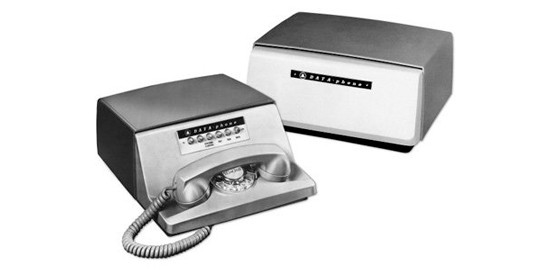
\includegraphics[scale=0.5, fbox={\fboxrule} 4mm]{images/03-antecedentes/09-modem_bell.jpg}
\caption{Módem Bell. 1958}
\label{fig:bell_modem}
\end{figure}

En el año 1972 al calor de una enorme y exitosa demostración de \ac{ARPANET}, se introduce la primera gran aplicación de esta nueva tecnología, el correo electrónico. Ray Tomlinson, había desarrollado para \ac{ARPANET} unos años antes un programa llamado SNDMSG para enviar mensajes entre las distintas terminales de una computadora, por lo que adaptó este programa para permitir el envío dentro de una red más amplia.

Con el crecimiento de la red, se desarrollaron tres protocolos que actualmente siguen en uso, \ac{TCP}, \ac{IP} y \ac{DNS}. El año 1983, \ac{ARPANET} se abre definitivamente a la vida civil permitiendo el intercambio masivo de datos entre universidades y centros de investigación. Este es el motivo último por el que se celebra ese año como el nacimiento de Internet.

La \textit{web} (\ac{www}) es probablemente el punto más visible de Internet. Fue desarrollado entre 1989 y 1990 por Tim Berners-Lee y Robert Cailiau mientras trabajaban en el \ac{CERN}.

En la web, es utilizado \ac{HTTP} como protocolo de comunicación, que define la sintaxis y la semántica necesarias para el correcto funcionamiento de los distintos componentes de la comunicación web, consiguiendo una abstracción que permite unificar la forma de comunicación en la red. En las comunicaciones en red el modelo de arquitectura más extendido es el paradigma Cliente - Servidor (ver figura \ref{fig:cliente-servidor}), mediante el cual se define una máquina \textit{servidor} encargada de generar la corriente datos y una serie de máquinas conocidas como \textit{clientes}, que realizan peticiones para consumir estos datos. El funcionamiento básico de este modelo podría verse como una farmacia abierta 24 horas (servidor), que está permanentemente a la espera de que alguna persona decida entrar a comprar algún medicamento, momento en el cual busca la droga pedida y se la facilita.

\begin{figure}[h!btp]
\centering
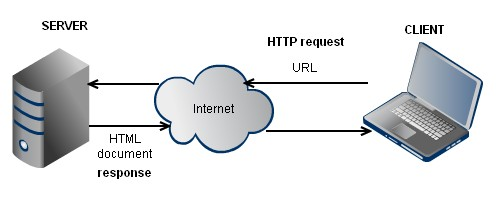
\includegraphics[scale=0.75, fbox={\fboxrule} 4mm]{images/03-antecedentes/10-client_server.png}
\caption{Modelo cliente-servidor}
\label{fig:cliente-servidor}
\end{figure}

Para que estas transacciones puedan darse, los computadores deben poder conocer como comunicarse, lo que en este caso se logra mediante las direcciones \ac{IP}, que consisten en una serie de 32 bits que designan unívocamente un elemento de una red, y unos pocos pasos intermedios, y transparentes para el usuario. El cliente, normalmente mediante un navegador web, es decir, mediante un programa creado específicamente para la navegación y visualización de páginas web, introduce el nombre de la página con la que quiere comunicarse. Este nombre, por ejemplo, \textit{www.usipv6.com}, es enviado automáticamente a unos servidores llamados servidores \ac{DNS}, que son capaces de buscar la dirección \ac{IP} asociada al nombre de la página tecleada y devolverla, que en este ejemplo es \textit{123.45.67.89} (ver figura \ref{fig:dns-server}). Es fácil ver el porqué se utiliza este paso intermedio, debido a que al usuario le resultará mucho más sencillo recordar una página web que una serie de números. Una vez realizada la traducción, el computador se comunica con el servidor a través de la dirección \ac{IP} obtenida y este le responde enviándole la información solicitada.

\begin{figure}[h!btp]
\centering
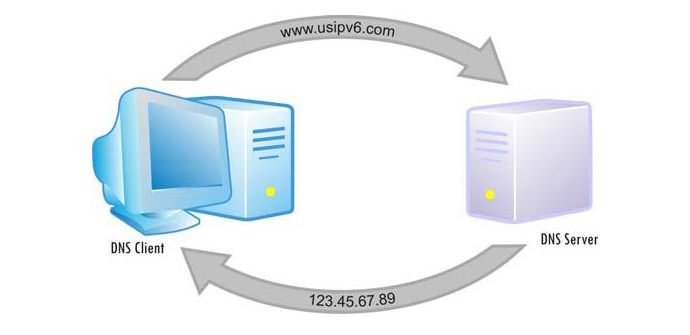
\includegraphics[scale=0.5, fbox={\fboxrule} 4mm]{images/03-antecedentes/11-dns_server.png}
\caption{Comunicación con servidor DNS}
\label{fig:dns-server}
\end{figure}

Aunque en sus orígenes la web se desarrolló para transmitir únicamente texto, actualmente, como puede verse fácilmente, se permite la emisión de todo tipo de contenidos multimedia, como audio, vídeo o imágenes. La tarea del cliente consiste en recibir los datos enviados por el emisor para reinterpretarlos y mostrarlos de manera coherente para el usuario.

Todo esto nos lleva a poder diferenciar de forma clara dos trabajos distintos dentro de la comunicación web, el trabajo llevado a cabo por el cliente y el trabajo llevado a cabo por el servidor. Para poder desarrollar cada una de estas tareas, existen una serie de tecnologías específicas para el lado del cliente y para el lado del servidor.

\subsection{Tecnologías del lado del servidor}
Como se ha explicado en la sección anterior, el servidor es el encargado de atender las peticiones que los clientes le envían y responderlas adecuadamente. 
En los comienzos de la web los servidores eran meras estaciones de \textit{almacenaje}, que devolvía al cliente peticionario una página web estática (ver figura \ref{fig:static-server}) mientras que en la actualidad, los servidores son capaces de generar el contenido que deben enviar de forma dinámica (ver figura \ref{fig:dynamic-server}).

\begin{figure}[h!btp]
\centering
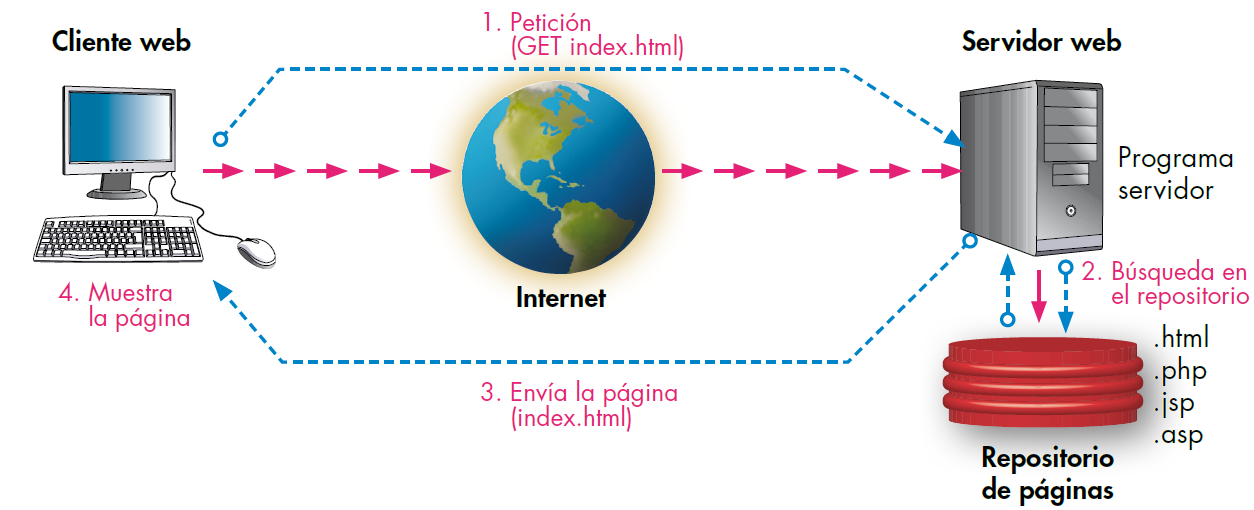
\includegraphics[scale=0.4, fbox={\fboxrule} 4mm]{images/03-antecedentes/12-html_request.png}
\caption{Petición a servidor estático}
\label{fig:static-server}
\end{figure}

\begin{figure}[h!btp]
\centering
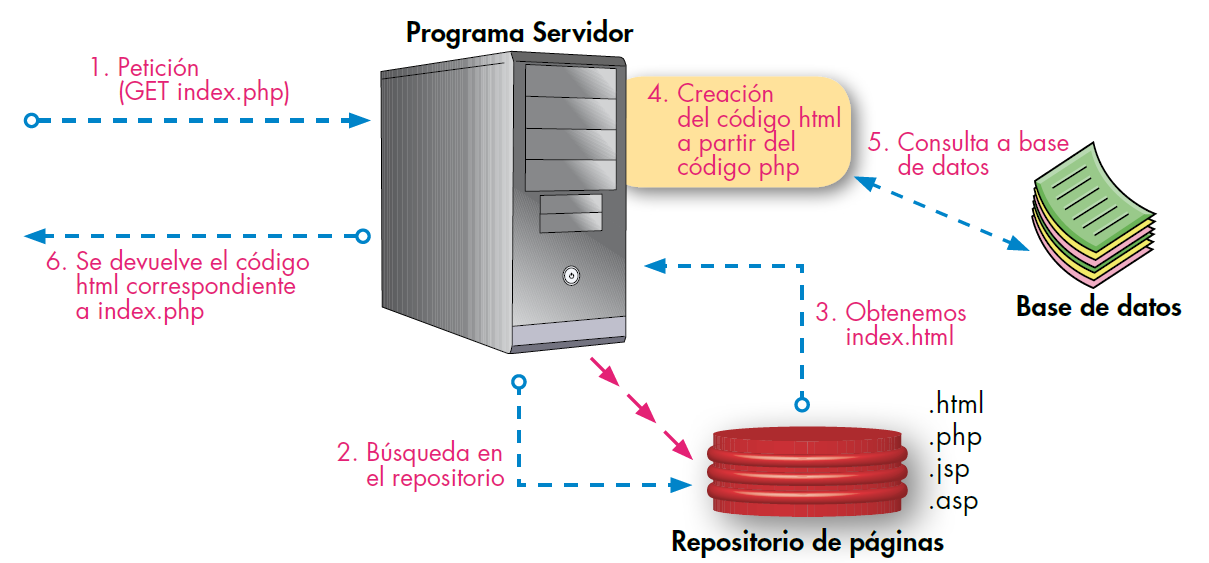
\includegraphics[scale=0.5, fbox={\fboxrule} 4mm]{images/03-antecedentes/13-html_dynamic_request.png}
\caption{Petición a servidor dinámico}
\label{fig:dynamic-server}
\end{figure}

Algunas de las tecnologías más utilizadas en el lado del cliente son Apache, PHP y MySQL.

Apache es un software que permite a un computador realizar el comportamiento típico de un servidor, esto es, atender a las peticiones de los clientes, ofrecerles servicios y enviarles la información pedida. Está desarrollado en C y es de código abierto \cite{Apac15}.

PHP es uno de los lenguaje de programación del lado del servidor más extendido y fue uno de los primeros en poder incorporarse directamente en el código \ac{HTTP}. Fue creado por Rasmus Lerdorf en 1994 y actualmente se encuentra en su versión 5.6.14 \cite{Hist15}.

MySQL es un sistema de gestión de bases de datos relacionales desarrollado para MySQL AB (actualmente parte de Sun Microsystems) en 1995 por Michael Widenius, David Axmark and Allan Larsson \cite{Data14}.

\begin{figure}[h!btp]
	\begin{adjustbox}{minipage=\linewidth, fbox}
		\centering
		\subfigure[MySQL]{
\includegraphics[scale=0.5]{./images/03-antecedentes/14-mysql.png}}
		\hspace{10mm}
		\subfigure[PHP]{
\includegraphics[scale=0.5]{./images/03-antecedentes/15-php.png}}
		\vspace{10mm}
		\subfigure[Apache]{
\includegraphics[scale=0.5]{./images/03-antecedentes/16-apache.png}}
	\end{adjustbox}
	\caption{Tecnologías utilizadas en servidores}
	\label{fig:mysql_php_apache}
\end{figure}

\subsection{Tecnologías del lado del cliente}
Dejando de lado la necesidad de contar con un navegador web que permita mostrar e interactuar con las páginas web, el cliente debe interpretar los datos recibidos por el servidor de manera que pueda traducirlos convirtiéndolos en el concepto de \textit{página web} que conocemos. Tres de los lenguajes más utilizados en este intercambio de datos son \ac{HTML}, \ac{CSS}, JavaScript y \ac{AJAX}.

\ac{HTML} es un lenguaje de marcado que se utiliza para la representación visual de una página web. Está considerado el lenguaje de programación más importante y está a cargo de la \ac{W3C} \cite{Worl15}. Aunque permite dar formato al texto, actualmente esto suele ser responsabilidad de las hojas \ac{CSS}.

La última versión de este lenguaje, \ac{HTML}5, publicada en octubre de 2014 \cite{Adam14} incorpora novedades como etiquetas con \ac{codec}, para manejar grandes conjuntos de datos o mejoras en los formularios.

\ac{CSS} es usado para definir el formato de una página web escrita en \ac{HTML}.


\begin{lstlisting}[
  float=ht,
  language = HTML,
  caption  = {«Hola mundo» en HTML y CSS},
  label    = code:hello]
	<!DOCTYPE html>
	<html>
	<head>
	    <title>Hola Mundo en HTML</title>
		<style>
		body {background-color:lightgrey}
		h1   {color:blue}
		p    {color:green}
		</style>
	</head>
	<body>
		<h1>Hola Mundo</h1>
		<p>Mi primera web en HTML y CSS.</p>
	</body>
	</html>
\end{lstlisting}

Javascript es un lenguaje interpretado orientado a objetos implementado normalmente como parte del navegador web.
 \ac{AJAX} es utilizado para poder realizar peticiones a un servidor modificando partes concretas de una página, eliminando de esta forma la necesidad de recargar la página completa.

% Desarrollo web (frameworks)


\section{Dispositivos móviles}
Los teléfonos móviles han cambiado nuestra manera de relacionarnos tanto con el mundo como entre las personas. Hace apenas diez años era imposible pensar en acceder a Internet desde cualquier lugar o tener la posibilidad de enviar mensajes a través de 
aplicaciones de mensajería instantánea. Hace veinte o treinta años nadie imaginaba que los teléfonos móviles serían un elemento imprescindible y omnipresente de nuestras vidas ya que en aquella época era un símbolo de estatus y gran lujo.

Podríamos comenzar a explicar los intentos de comunicarse a través de grandes distancias con el telégrafo, primer gran antecedente del teléfono, y es que este invento fue algo revolucionario cuando se presentó. Por primera vez spermitía comunicar dos puntos distantes de manera instantánea.

Los orígenes del telégrafo se remontan al S. XVIII cuando Claude Chappe desarrolló para el ejército Francés su precursor inmediato, el telégrafo óptico. Este invento consistía en un sistema de comunicación que emitía una señal visual que podía repetirse en la distancia, aunque solo tenía utilidad en las distancias en las que el ojo humano permitía distinguirlas (ver figura \ref{fig:telegrafo_optico}) \cite{Holz94}.

\begin{figure}[h!btp]
	\begin{adjustbox}{minipage=\linewidth, fbox}
		\centering
		\subfigure[Telégrafo óptico de Claude Chappe]{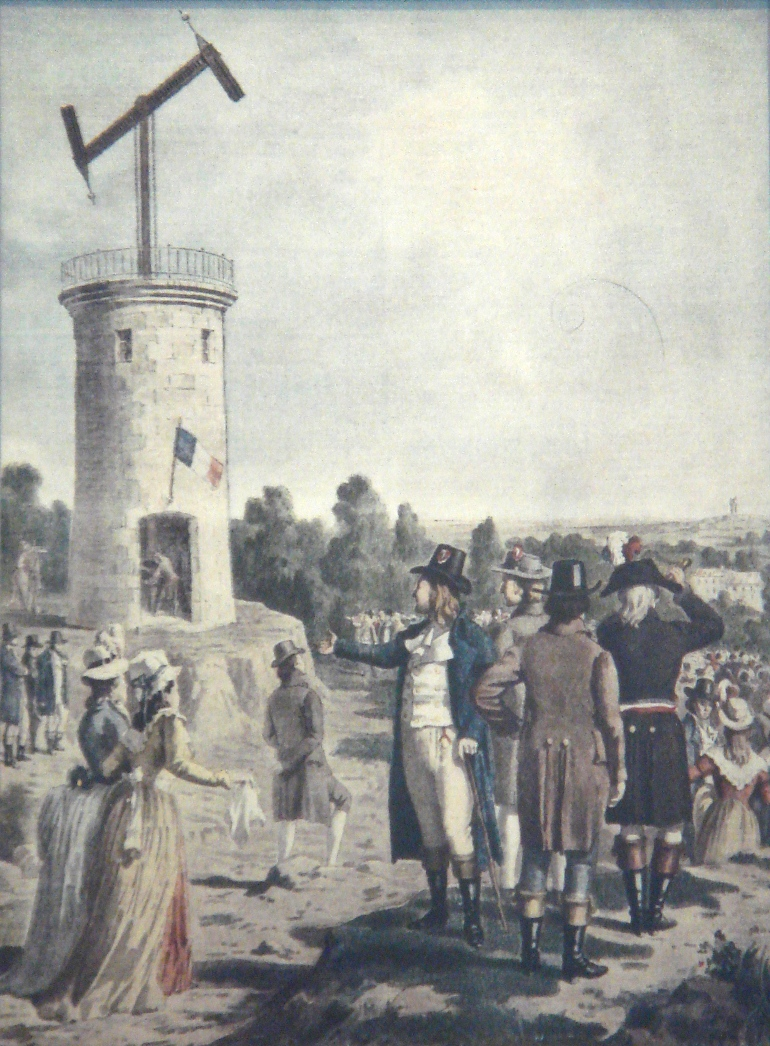
\includegraphics[height=80mm]{./images/03-antecedentes/17-telegrafo_optico.jpg}}
		\hspace{10mm}
		\subfigure[Claude Chappe]{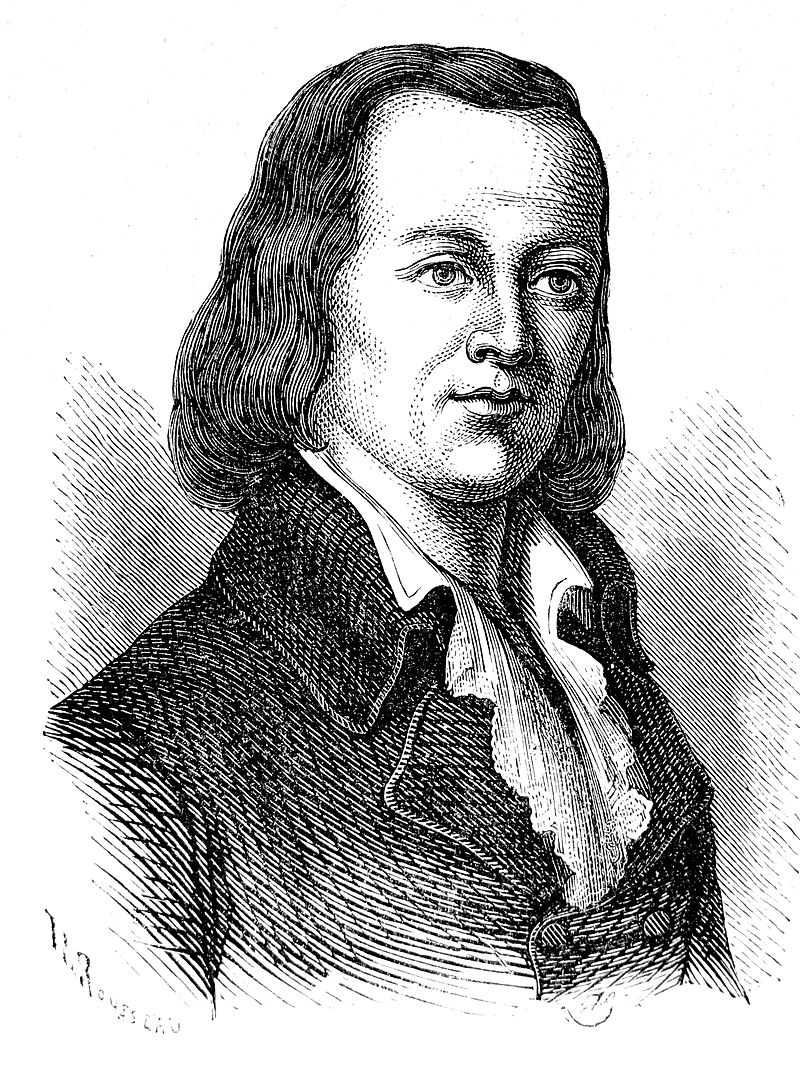
\includegraphics[height=80mm]{./images/03-antecedentes/18-claude_chappe.jpg}}
	\end{adjustbox}
\caption{Telégrafo óptico}
	\label{fig:telegrafo_optico}
\end{figure}

Con la intención de mejorar el alcance de la comunicación y aprovechando los estudios de electromagnetismo de Michael Faraday y las innovaciones de William Sturgeon y Joseph Henry sobre el electroimán, Samuel Morse (ver figura \ref{fig:telegrafo}) ideó una manera de enviar señales entre dos puntos aprovechando las corrientes eléctricas. En un primer momento, el telégrafo consistía en un péndulo que ante la existencia de corriente movía un lápiz que dibujaba de esa manera una línea sobre un papel. Mejorando el prototipo se llegó a inventar el famoso código morse, que consta de los consabidos y famosos dos elementos: el punto y la raya.

\begin{figure}[h!btp]
	\begin{adjustbox}{minipage=\linewidth, fbox}
		\centering
		\subfigure[Samuel Morse]{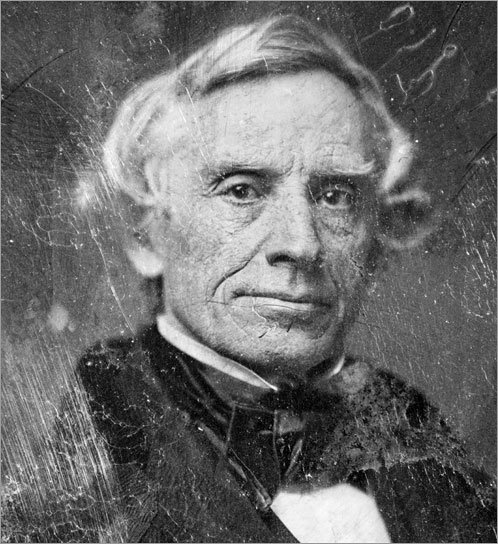
\includegraphics[height=80mm]{./images/03-antecedentes/20-samuel_morse.jpg}}
		\hspace{10mm}
		\subfigure[Código morse]{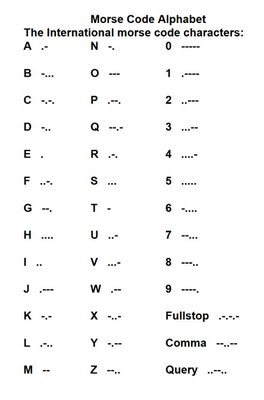
\includegraphics[height=80mm]{./images/03-antecedentes/21-codigo_morse.jpg}}
	\end{adjustbox}
\caption{Código Morse}
	\label{fig:telegrafo}
\end{figure}

En 1837 Samuel Morse hizo la primera demostración pública del telégrafo en un áula de la universidad de Nueva York. 

El 24 de mayo de 1844, se terminó la línea telegráfica que unía Baltimore y Washington, enviando un mensaje desde la Cámara de la Corte Suprema en el Capitolio de \ac{EE.UU.} en Washington hasta el ferrocarril B \& O en Baltimore con la frase \textit{What hath God wrought?} perteneciente al libro de los Números (ver figura \ref{fig:telegrama}).

\begin{figure}[h!btp]
\centering
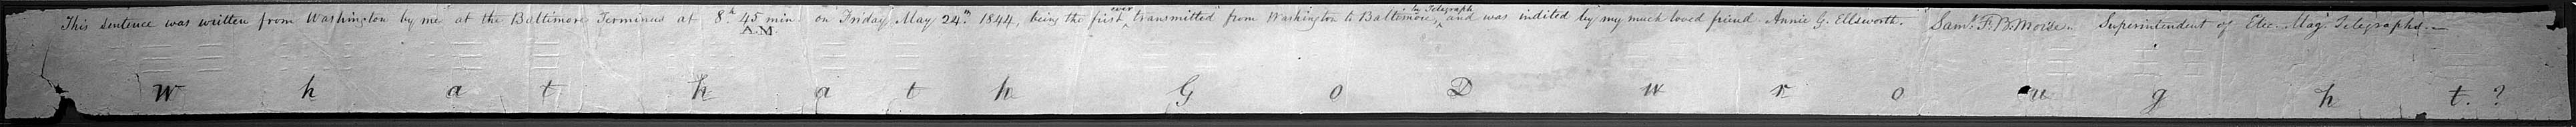
\includegraphics[width=100mm, fbox={\fboxrule} 4mm]{images/03-antecedentes/19-primer_telegrama.jpg}
\caption{Primer telegrama}
\label{fig:telegrama}
\end{figure}

El siguiente gran paso en las comunicaciones viene de la mano de un dispositivo capaz de retransmitir, a través de cables, las señales acústicas derivadas de la voz humana. El teléfono.

Históricamente, la invención del teléfono se atribuyó a Alexander Graham Bell \cite{Cab79}, hasta  el 11 de junio de 2002, fecha en que fue reconocido el italiano Antonio Meucci (ver figura \ref{fig:telefono}) como el verdadero inventor de este aparato por el Congreso de los Estados Unidos \cite{Uni03}.

\begin{figure}[h!btp]
	\begin{adjustbox}{minipage=\linewidth, fbox}
		\centering
		\subfigure[Antonio Meucci]{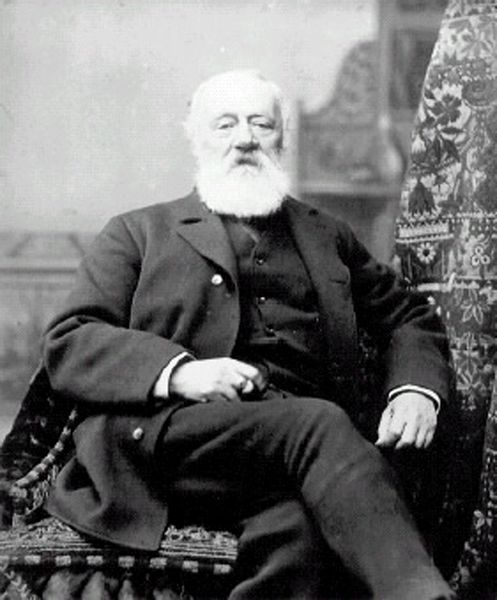
\includegraphics[height=80mm]{./images/03-antecedentes/22-antonio_meucci.jpg}}
		\hspace{10mm}
		\subfigure[Alexander Graham Bell]{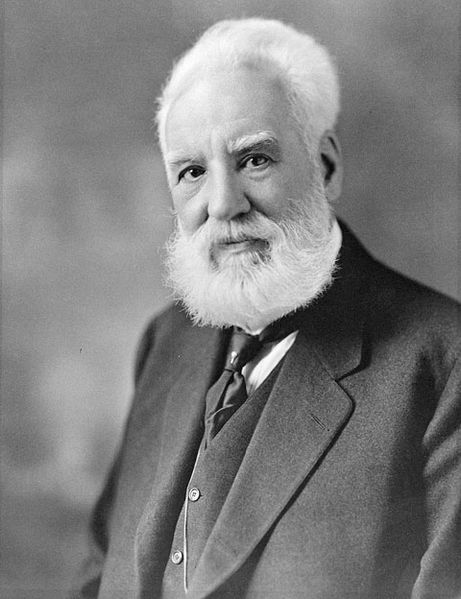
\includegraphics[height=80mm]{./images/03-antecedentes/23-alexander_graham_bell.jpg}}
	\end{adjustbox}
\caption{Inventores del teléfono}
	\label{fig:telefono}
\end{figure}

Antonio Meucci, nacido en Florencia, emigró junto a su esposa Ester Mochi primero a Cuba en octubre de 1835 y después a Staten Island, Nueva York \ac{EE.UU.} en 1850.

Ya que vivían en una casa de varios pisos y a causa del reumatismo de su esposa, Meucci construyó el primer teléfono para comunicar su despacho, situado en la planta baja, con el dormitorio, ubicado en el piso superior, donde se encontraba postrada su esposa debido a la enfermedad. Esto ocurrió alrededor de 1857 \cite{Meuc10}. El 28 de diciembre de 1871 presentó la documentación previa a la patente, pero sólo consiguió el dinero para renovarla en 1872 y 1873. Meucci ofreció una demostración de su \textit{teletrófono} a la \textit{Western Union Telegraph Company} pero viendo la falta de interés de la empresa en su desarrollo, pidió la devolución de los materiales presentados, recibiendo como única contestación la explicación de que habían sido perdidos y por tanto no resultaba  posible su devolución.

Aunque este hecho no está probado, parece ser que estos materiales cayeron en manos de Alexander Graham Bell, que en aquella época trabajaba en los laboratorios de la compañía, utilizándolos más tarde para desarrollar su propio teléfono. En 1876 Bell presentó, unas horas antes que su compatriota Elisha Gray, la patente de su teléfono. 

Ante las reclamaciones de Meucci de la autoría del invento, y gracias a la intervención de un amigo, se descubrió que las patentes relacionadas con el \textit{telégrafo parlante}, se habían \textit{extraviado}. En investigaciones posteriores se descubrieron pagos a funcionarios por parte de Bell para hacer desaparecer estos documentos. Debido a las pruebas de prevaricación, en 1886 el Secretario de Estado llegó a confirmar que existían suficientes pruebas para otorgar la autoría del invento a Antonio Meucci. La demanda cesó como consecuencia de la muerte de Meucci en octubre de 1889, después de que los abogados de Bell consiguieran dilatar el proceso mediante recursos judiciales. Como curiosidad, Thomas Alva Edison enviaría una carta al juez posicionándose a favor de Meucci en sus reivindicaciones \cite{Carb07}.

\begin{figure}[h!btp]
	\begin{adjustbox}{minipage=\linewidth, fbox}
		\centering
		\subfigure[Teléfono de Meucci]{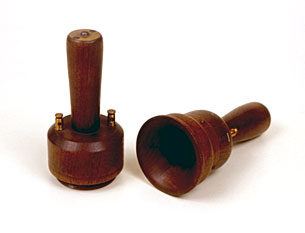
\includegraphics[scale=0.5]{./images/03-antecedentes/24-telefono_meucci.jpg}}
		\hspace{10mm}
		\subfigure[Teléfono de Bell]{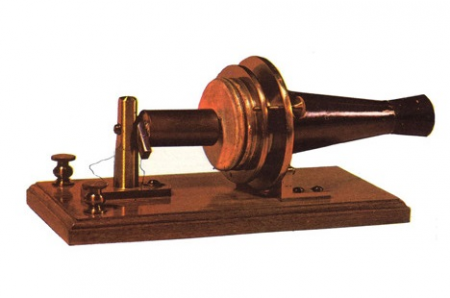
\includegraphics[scale=0.5]{./images/03-antecedentes/25-telefono_bell.png}}
	\end{adjustbox}
	\caption{Primeros teléfonos}
	\label{fig:primeros-telefonos}
\end{figure}


El 9 de octubre de 1876 se realizó una demostración en la que Bell y su ayudante Thomas Watson mantuvieron una conversación telefónica entre Cambridge y Boston. La primera frase pronunciada durante este evento fue \textit{''Mr. Watson, come here. I want to see you.''} \cite{Even01}.

Dejando de lado los primeros intentos de radiotelefonía, el primer teléfono móvil fue desarrollado por Motorola en 1983. El modelo \ac{DynaTAC} 8000x que tenía una autonomía de 1 hora y permitía treinta minutos de conversación. El precio de venta al público se estableción en casi 4.000 dólares.

Aunque la comercialización se llevo a cabo en la  mencionada fecha, la primera llamada se realizó diez años antes, en abril de 1973 por Martin Cooper, director de Motorola al teléfono fijo de Joel Engel, investigador de los laboratorios Bell, su principal competidora. En una entrevista para la BBC, Cooper comentaba cómo se desarrolló esa primera conversación: ''Joel it's Martin and i'm calling you from a cell phone, but a real cell phone'' \cite{BBC13}\footnote{Cómo curiosidad se incluye el enlace al vídeo promocional del DynaTAC 8000X \url{https://www.youtube.com/watch?v=0WUF3yjgGf4}}.

\begin{figure}[h!btp]
	\begin{adjustbox}{minipage=\linewidth, fbox}
		\centering
		\subfigure[Motorola DynaTAC 8000X]{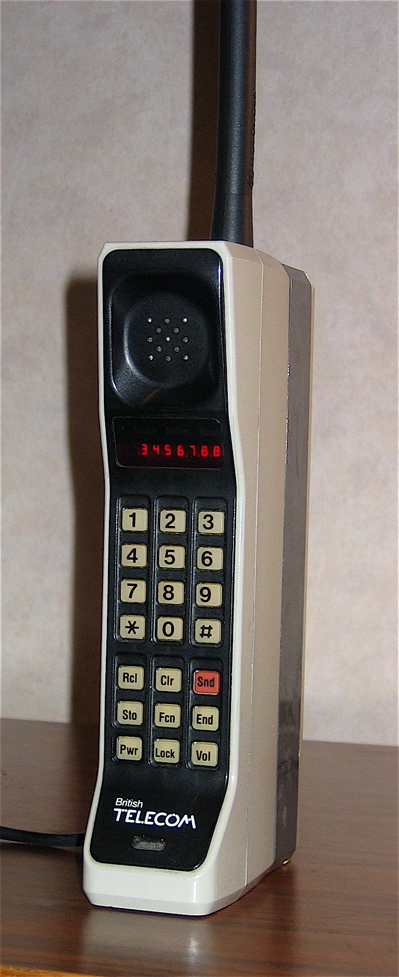
\includegraphics[height=45mm]{./images/03-antecedentes/27-motorola-dynatac_8000x.jpg}}
		\hspace{10mm}
		\subfigure[Martin Cooper]{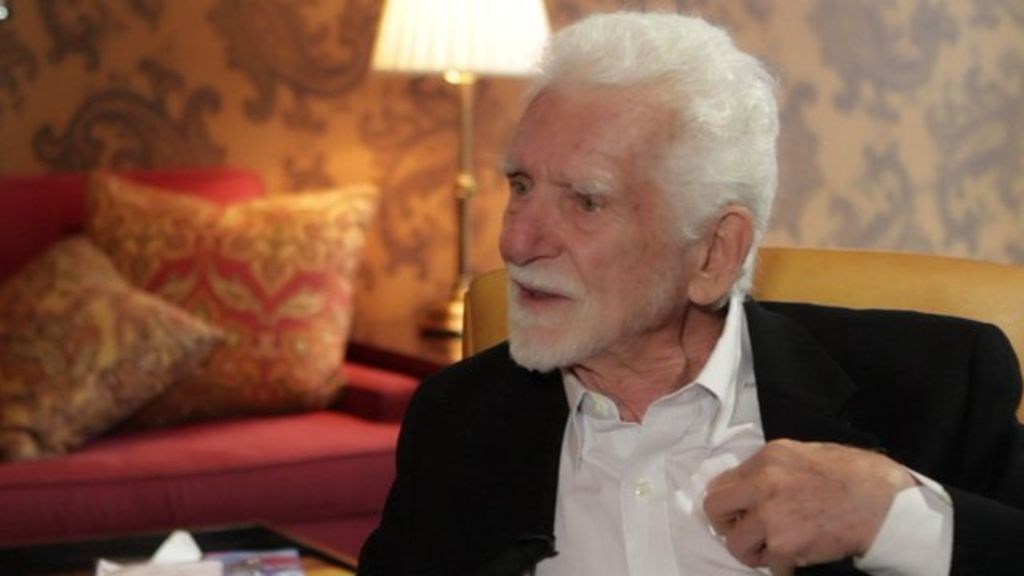
\includegraphics[width=80mm]{./images/03-antecedentes/28-martin_cooper.jpg}}
	\end{adjustbox}
\caption{Primeros teléfonos}
	\label{fig:primeros-telefonos2}
\end{figure}

La gran novedad de estos primeros modelos sobre los aparatos de radiotelefonía es que podían ser trasladados y manejados por una sola persona, ya que hasta ese momento únicamente estaban disponibles modelos de gran tamaño y peso que debían transportarse en los maleteros de los vehículos.

La primera generación de teléfonos móviles fue desarrollada hasta finales de los años 80. Estos primeros modelos únicamente permitían el intercambio de voz.

La segunda generación llego en los años 90, poniendo el acento en la digitalización de las comunicaciones, ya que ofrecían un aumento sustancial de la calidad de voz y se simplificaba la fabricación reduciendo los costes. En este momento se integró uno de los servicios más populares de los teléfonos móviles hasta la aparición de la mensajería instantánea, los \ac{SMS}.

\begin{figure}[h!btp]
\centering
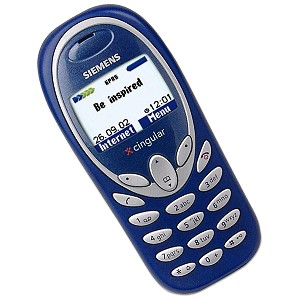
\includegraphics[height=40mm, fbox={\fboxrule} 4mm]{images/03-antecedentes/29-siemens_a56.jpg}
\caption{Teléfono de segunda generación. Siemens A56}
\label{fig:siemens-a56}
\end{figure}

El siguiente gran salto vino de la mano de Apple y su iPhone, sacado al mercado en el año 2007. Con un diseño estudiado y una pantalla multitáctil, aprovechando la buena imagen de marca conseguida a través del iPod, Apple sacó un teléfono que revolucionó la manera en la que hasta entonces se entendían los teléfonos. Siendo una mezcla de teléfono, ordenador, reproductor de música, agenda personal y reproductor multimedia, no tardó en convertirse en un producto casi imprescindible para el consumidor y por tanto algo a imitar por las compañías rivales. Había nacido la era de los smartphones.

\begin{figure}[h!btp]
\centering
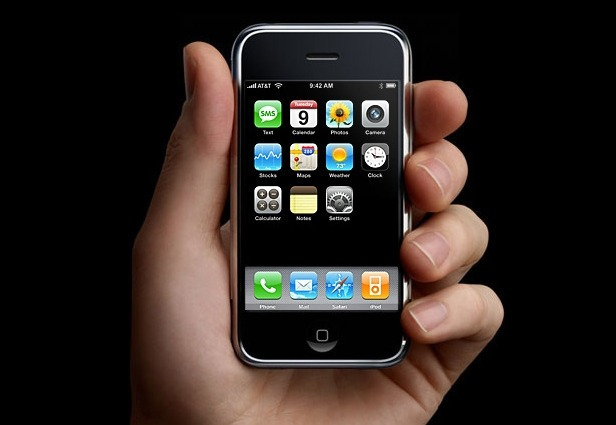
\includegraphics[width=60mm, fbox={\fboxrule} 4mm]{images/03-antecedentes/30-iphone.jpg}
\caption{iPhone de Apple}
\label{fig:iphone}
\end{figure}

\section{Aplicaciones similares}
En este apartado presentaremos aplicaciones similares a la que se pretende desarrollar. El parecido viene dado bien por el uso de la localización, bien por la compartición de la ubicación o bien por ser aplicaciones con la misma finalidad que la desarrollada en el presente \ac{TFG}.

\subsection{Foursquare}
Sin duda alguna, Foursquare (\url{https://es.foursquare.com/}) es la aplicación más conocida de las presentadas. Fue creada en 2009 por Dennis Crowley y Naveen Selvadurai. Básicamente consistía en una red social que permitía indicar el punto geográfico en el que el usuario se encuentra en ese momento \cite{Rubi13} y opinar acerca del lugar, establecimiento o comercio y mostrar los puntos de interés cercanos a su posición \cite{Cano14}. 

Esta aplicación está disponible para \href{https://play.google.com/store/apps/details?id=com.joelapenna.foursquared}{Android}, \href{https://itunes.apple.com/us/app/id306934924?mt=8}{iOS} y \href{https://www.microsoft.com/es-es/store/apps/foursquare/9wzdncrfhw3v}{Windows Mobile}.

\begin{figure}[h!btp]
	\begin{adjustbox}{minipage=\linewidth, fbox}
		\centering
		\subfigure[Aplicación Foursquare en funcionamiento]{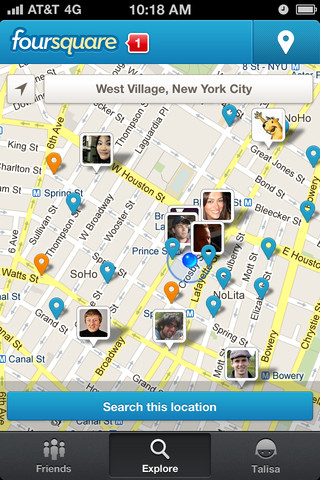
\includegraphics[scale=0.6]{./images/03-antecedentes/50-foursquare_app.jpg}}
		\hspace{10mm}
		\subfigure[Logo de Foursquare]{
\includegraphics[width=40mm, fbox={\fboxrule} 4mm]{images/03-antecedentes/38-foursquare.png}}
	\end{adjustbox}
\caption{Foursquare}
	\label{fig:foursquare}
\end{figure}

\subsection{Swarm}
En el año 2014 Foursquare lanza Swarm (\url{https://es.swarmapp.com/}), que es una escisión dedicada más a compartir la posición y permitir concertar lugares de encuentro y saber qué contactos tenemos cerca dejando de lado la parte lúdica y la compartición de experiencias, que se trasladan definitivamente a Foursquare \cite{Buzz14}.

Esta aplicación está disponible para \href{https://play.google.com/store/apps/details?id=com.foursquare.robin}{Android}, \href{https://itunes.apple.com/US/app/id870161082?mt=8}{iOS} y \href{https://www.microsoft.com/es-es/store/apps/swarm/9wzdncrdrsq1}{Windows Mobile}.

\begin{figure}[h!btp]
\centering

\includegraphics[scale=0.25, fbox={\fboxrule} 4mm]{images/03-antecedentes/39-swarm.png}
\caption{Logo de Swarm}
\label{fig:swarm}
\end{figure}

\subsection{Glympse}
Glympse (\url{https://www.glympse.com/}) es una aplicación que permite compartir en tiempo real la ubicación del usuario con los contactos que desee. Es una forma rápida de indicar y compartir la posición en la que te encuentras, viniendo a responder a la pregunta, ''¿Dónde te encuentras en este momento?'', sin necesidad de abrir el móvil. Los destinatarios de los ''Glympses'' no necesitan tener instalada la aplicación para acceder a nuestros recorridos \cite{Unk15}.

Esta aplicación está disponible para \href{https://play.google.com/store/apps/details?id=com.glympse.android.glympse}{Android}, \href{https://itunes.apple.com/app/glympse-share-gps-location/id330316698?mt=8}{iOS} y \href{https://www.microsoft.com/es-es/store/apps/glympse/9wzdncrdf9sj}{Windows Mobile}.

\begin{figure}[h!btp]
	\begin{adjustbox}{minipage=\linewidth, fbox}
		\centering
		\subfigure[Aplicación Glympse en funcionamiento]{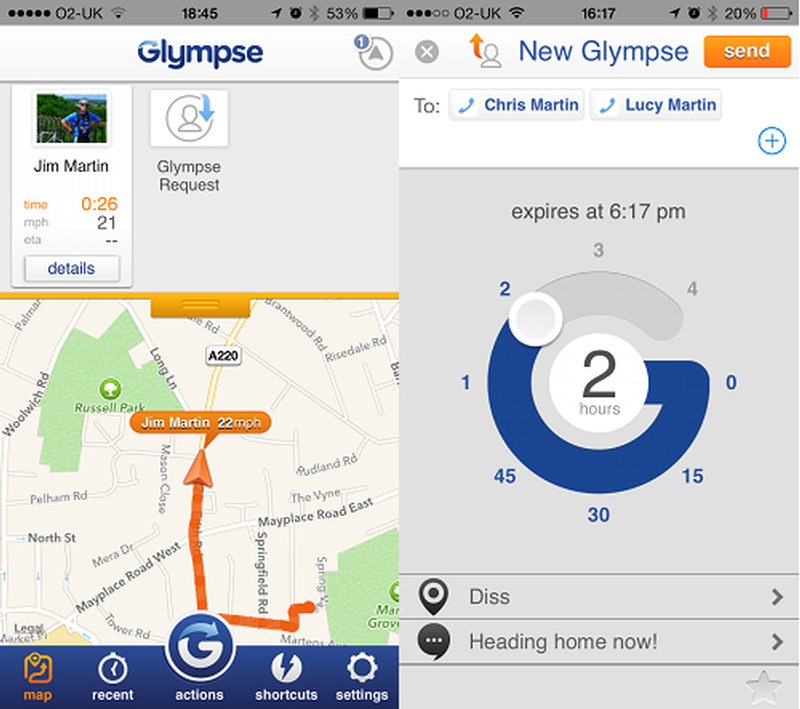
\includegraphics[scale=0.3]{./images/03-antecedentes/40-glympse_app.png}}
		\hspace{10mm}
		\subfigure[Logo Glympse]{
\includegraphics[width=40mm]{./images/03-antecedentes/41-glympse_logo.png}}
	\end{adjustbox}
\caption{Glympse}
	\label{fig:glympse}
\end{figure}

\subsection{Strava}
Strava (\url{https://www.strava.com/}) es una aplicación que permite hacer un seguimiento al usuario mientras realiza actividades deportivas. Permite el seguimiento entre usuarios y genera estadísticas de rendimiento que pueden ser comparadas. Puede utilizarse a través de la página web, sin necesidad de descargarse las distintas aplicaciones \cite{Moya12}.

Esta aplicación está disponible para \href{https://play.google.com/store/apps/details?id=com.strava}{Android} y \href{https://itunes.apple.com/app/strava-cycling/id426826309?mt=8}{iOS}.

\begin{figure}[h!btp]
	\begin{adjustbox}{minipage=\linewidth, fbox}
		\centering
		\subfigure[Aplicación Strava en funcionamiento]{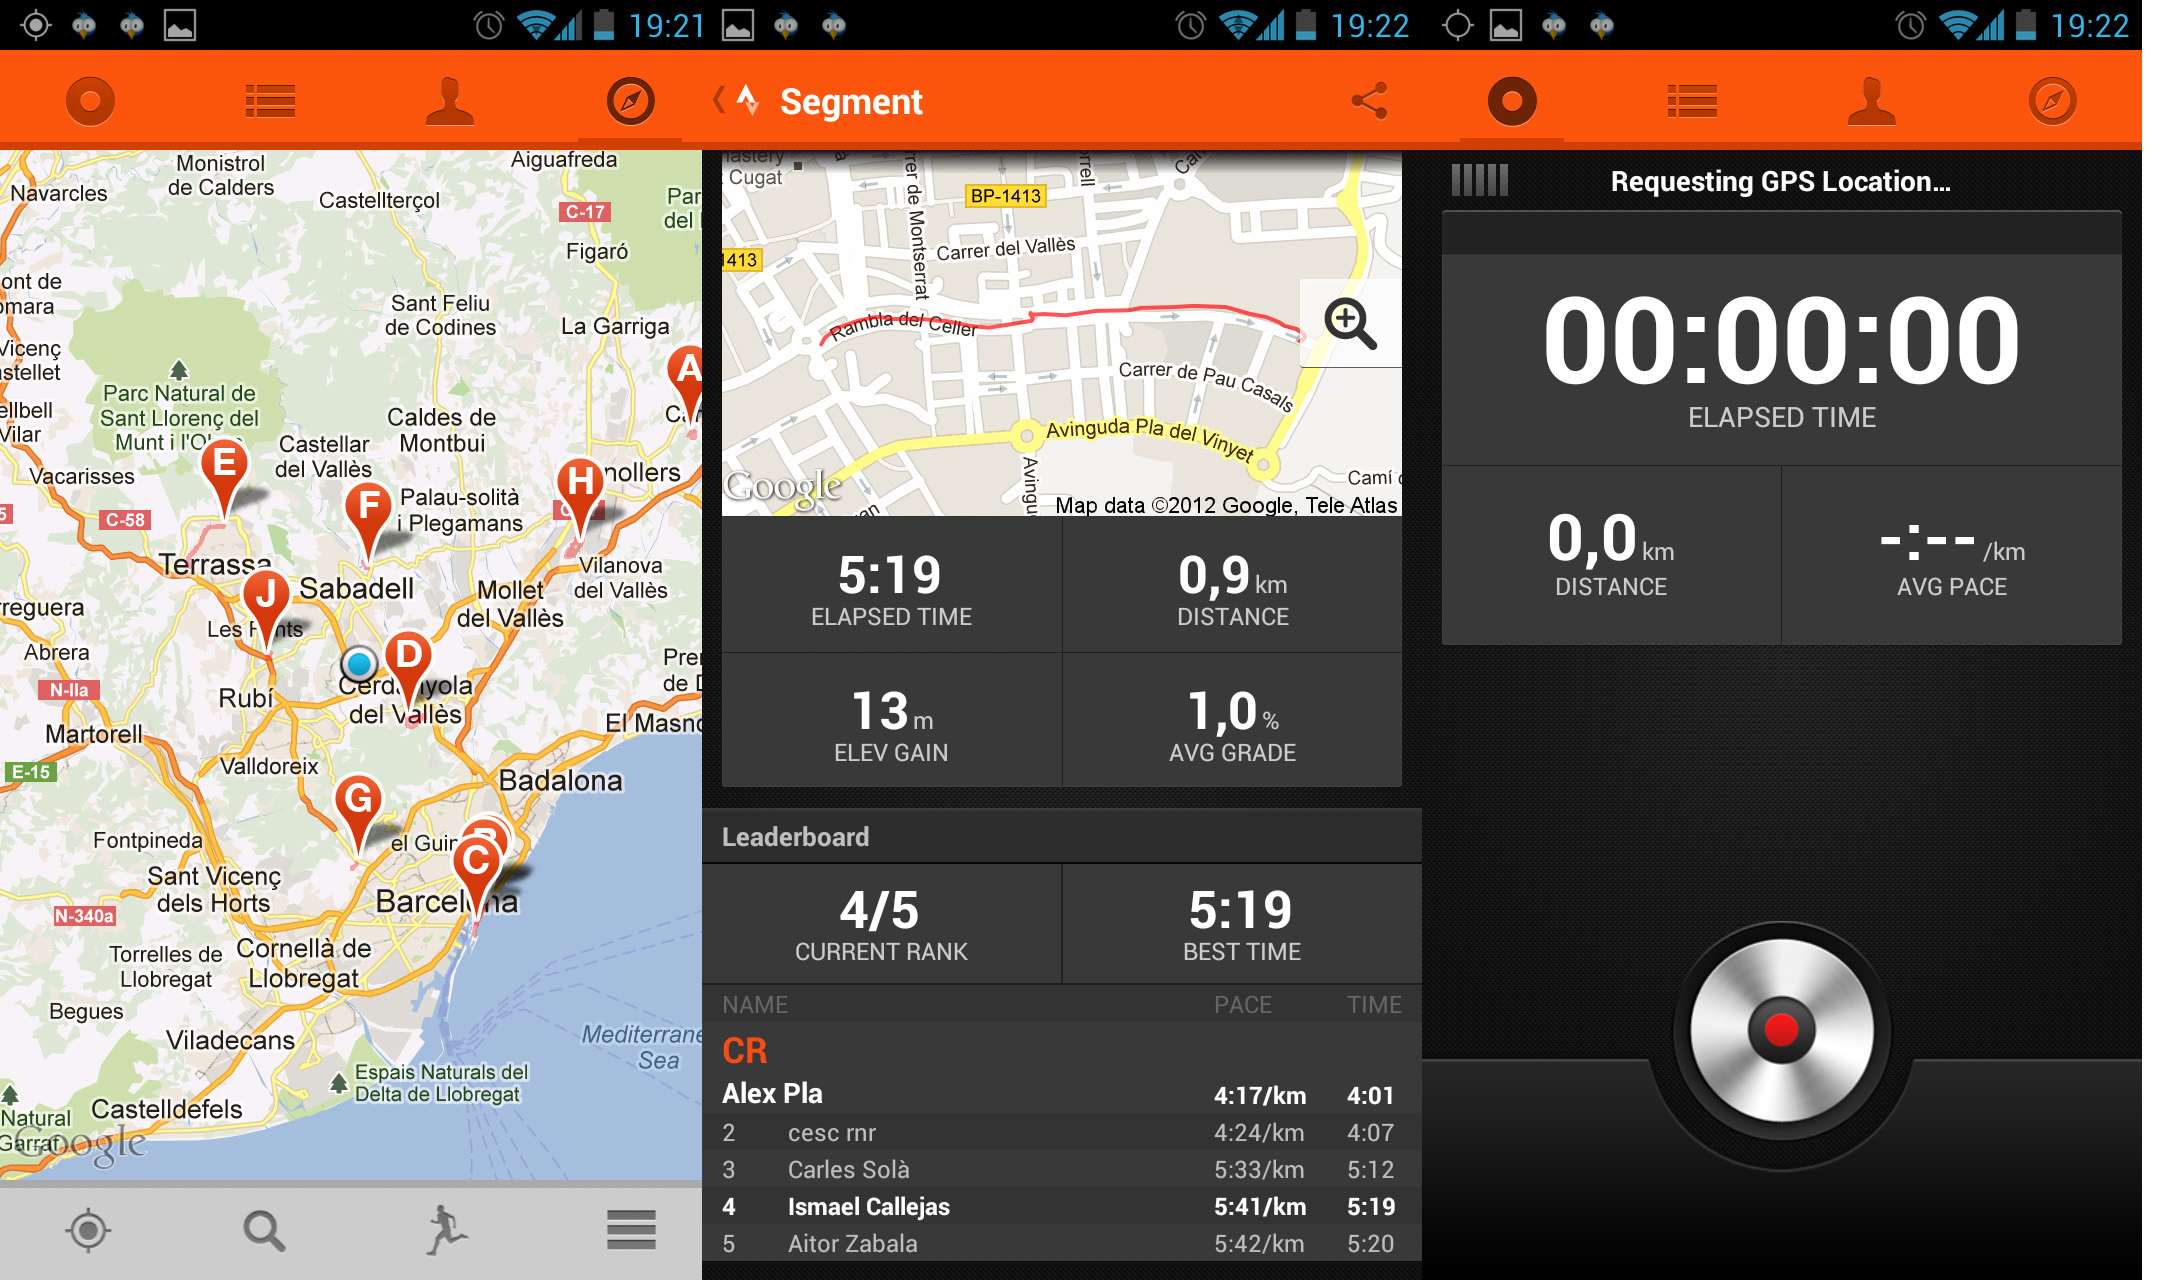
\includegraphics[width=120mm]{./images/03-antecedentes/42-strava_app.jpg}}
		\hspace{10mm}
		\subfigure[Logo Strava]{
\includegraphics[width=40mm]{./images/03-antecedentes/43-strava_logo.png}}
	\end{adjustbox}
\caption{Strava}
	\label{fig:strava}
\end{figure}

\subsection{Waze}
Waze (\url{https://www.waze.com/es/}) es una aplicación que permite compartir en tiempo real información sobre el estado del tráfico, de manera que el usuario recibe y envía el estado de las carreteras a todos aquellos usuarios de la comunidad conectados en ese momento. Permite adecuar las rutas de tráfico en función de los atascos detectados, informa de los precios de las gasolineras y permite avisar al resto de conductores de la posición de patrullas de tráfico o radares, último aspecto este que le ha dado gran controversia \cite{Cast13}. También permite interactuar automáticamente con Foursquare, marcando la posición de llegada justo al terminar el viaje, y con otras redes sociales como Facebook o Twitter \cite{Pen11}. A mediados de 2013 fue adquirida por Google por un total de 966 millones de dólares \cite{ABC13}.

Esta aplicación está disponible para \href{https://play.google.com/store/apps/details?id=com.waze}{Android}, \href{https://itunes.apple.com/us/app/waze-social-gps-traffic/id323229106?mt=8}{iOS} y \href{https://www.microsoft.com/es-es/store/apps/waze/9wzdncrfj2m3}{Windows Mobile}.

\begin{figure}[h!btp]
	\begin{adjustbox}{minipage=\linewidth, fbox}
		\centering
		\subfigure[Aplicación Waze en funcionamiento]{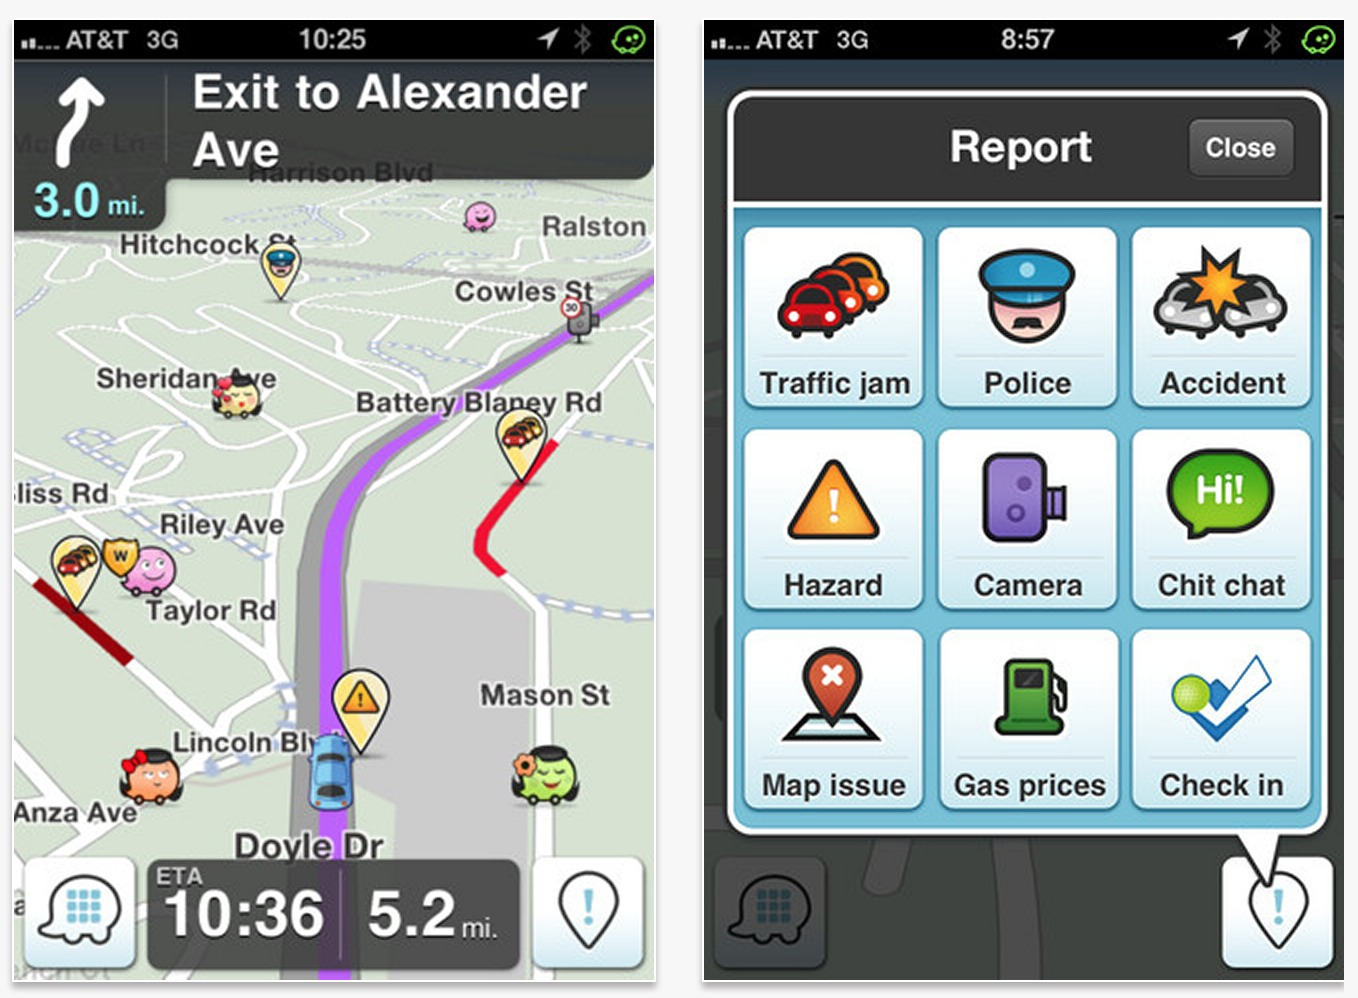
\includegraphics[scale=0.3]{./images/03-antecedentes/45-waze_app.jpg}}
		\hspace{10mm}
		\subfigure[Logo Waze]{
\includegraphics[width=40mm]{./images/03-antecedentes/44-waze_logo.png}}
	\end{adjustbox}
\caption{Waze}
	\label{fig:waze}
\end{figure}

\subsection{Ingress}

Como curiosidad del uso de los gps y la comunicación social, alejándonos de lo habitual, se encuentra Ingress (\url{https://www.ingress.com/}), un juego de realidad aumentada a través de gps que permite ''conquistar'' zonas de interés mientras estés cerca de ellas. Estas zonas normalmente coinciden con puntos emblemáticos y conocidos de las ciudades. La interacción social se consigue debido a que existen dos bandos enfrentados por conseguir los recursos de las zonas. Este juego está desarrollado por Niantic y distribuido por Google \cite{Pen13}.

Desde diciembre de 2013 está disponible para \href{https://play.google.com/store/apps/details?id=com.nianticproject.ingress}{Android} mientras que el lanzamiento para \href{https://itunes.apple.com/us/app/ingress/id576505181?mt=8}{iOS} fue en julio de 2014.

\begin{figure}[h!btp]
	\begin{adjustbox}{minipage=\linewidth, fbox}
		\centering
		\subfigure[Aplicación Ingress en funcionamiento]{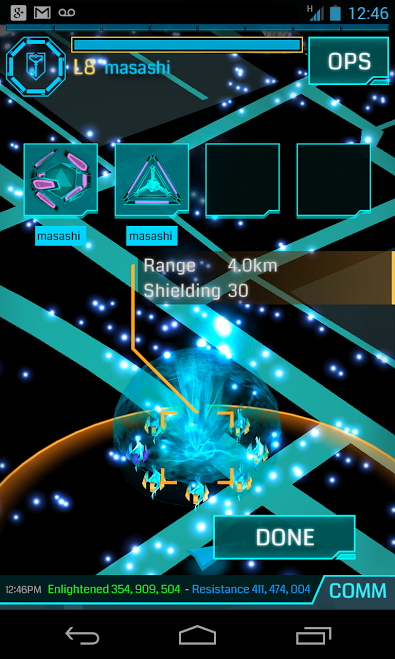
\includegraphics[height=80mm]{./images/03-antecedentes/46-ingress_app.png}}
		\hspace{10mm}
		\subfigure[Logo Ingress]{\includegraphics[width=40mm]{./images/03-antecedentes/47-ingress_logo.png}}
	\end{adjustbox}
\caption{Ingress}
	\label{fig:ingress}
\end{figure}

\subsection{Life360 Family Locator}
El concepto que subyace detrás de esta aplicación (\url{https://www.life360.com/family-locator/} es extremadamente sencillo, tener localizados en un mapa a todos los miembros de una familia mediante el gps del móvil \cite{Unk13}.

Esta aplicación está disponible para \href{https://play.google.com/store/apps/details?id=com.life360.android.safetymapd}{Android}, \href{https://itunes.apple.com/us/app/life360-locator/id384830320?mt=8}{iOS} y \href{https://www.microsoft.com/es-es/store/apps/life360-family-locator/9wzdncrfj0gw}{Windows Mobile}.

\begin{figure}[h!btp]
	\begin{adjustbox}{minipage=\linewidth, fbox}
		\centering
		\subfigure[Aplicación Life360 Family Locator en funcionamiento]{\includegraphics[height=80mm]{./images/03-antecedentes/48-life360_app.jpg}}
		\hspace{10mm}
		\subfigure[Logo Life360 Family Locator]{\includegraphics[width=40mm]{./images/03-antecedentes/49-life360_logo.png}}
	\end{adjustbox}
\caption{Life360 Family Locator}
	\label{fig:life360}
\end{figure}

\subsection{¿Dónde está mi coche?}
Esta aplicación guarda la ubicación marcada por el gps del móvil en cuanto pierda la conexión bluetooth con del coche \cite{Unk14}.

Está disponible para \href{https://play.google.com/store/apps/details?id=com.whereismycar&hl=es}{Android} e \href{https://itunes.apple.com/es/app/donde-esta-mi-coche/id504186557?mt=8}{iOs}.

\subsection{Find my car}
Aplicación que almacena la posición indicada por el gps del móvil cuando el usuario lo solicita. Permite acciones secundarias como cronometrar el tiempo que pasa desde que has aparcado, mostrar el camino de vuelta o sacar fotos del lugar de aparcamiento \cite{Unk14}.

Está disponible para \href{https://play.google.com/store/apps/details?id=com.elibera.android.findmycar&hl=es}{Android} e \href{https://itunes.apple.com/us/app/find-my-car/id349510601?mt=8}{iOs}.

% Local Variables:
%  coding: utf-8
%  mode: latex
%  mode: flyspell
%  ispell-local-dictionary: "castellano8"
% End:
